\chapter{Parametric study of impact of vegetation}
\label{ch:parametricstudy}
\def\figdir{chapters/ch03_numericalmodelsimple/figures}

\textit{This chapter is based on paper \cite{Manickathan2018a}}.
	

\section{Introduction}

%Cities are known to experience higher temperatures than the surrounding rural areas (Oke, 1973). This Urban Heat Island (UHI) effect has detrimental effects on human health and comfort in cities (Santamouris and Asimakopoulos, 2001). Furthermore, in the future, the UHI effect will grow due to increasing urbanization, which will lead to a predicted urban population of 5 billion by 2030 and 66% of the world’s population living in cities by 2050 (Seto et al., 2012; United Nations, 2015). The temperatures in urban areas will further increase due to the combined effect of climate change with a projected 2-4 ℃ increase in global average surface temperature by 2100 (Pachauri et al., 2014). Vegetation can provide cooling and is therefore increasingly being considered as part of UHI mitigation strategies to improve the human comfort in cities.

\lettrine[lines=3,nindent=0em,loversize=0.1]{I}{n} this chapter, a parametric study of the influence of environmental factors and tree properties on the transpirative cooling effect of a single row of trees is presented. The environmental factors investigated are wind speed, relative humidity, air temperature and solar radiation. The tree properties investigated are stomatal resistance, leaf size and leaf area density. In addition, the influence of vegetation size in the domain is studied by varying tree height and number of tree rows. The study aims at answering the following key questions: How does the climate influence the transpirative cooling effect of a single row of trees? Which features of the trees improve its cooling performance? Does increasing the size of the vegetated volume consistently improve the cooling of the environment? These findings can then assist in developing specific guidelines for effective UHI mitigation measures. To the author’s knowledge, few rigorous studies have been performed to investigate the cooling effect of individual trees. 

%The effectiveness of vegetation as a UHI mitigation strategy has been verified through various field measurements including on-site survey and remote sensing studies. Bowler et al. (2010) provide an extensive review of such empirical studies summarizing the effectiveness of parks, trees, ground vegetation and green roofs on the urban climate. These studies show that vegetation prevents warming of land surfaces and the air through evapotranspiration and shading. For example, parks and trees are shown to provide a cooling on average around 0.5 to 3 ℃ to cities (Bowler et al., 2010; Chen and Wong, 2006; Kurn et al., 1994; Ng et al., 2012; Rahman et al., 2017). However, it is also seen that the cooling provided by vegetation is dependent on the local climate, vegetation species and the amount of vegetation. Numerical simulation using urban microclimate models can, therefore, be an important mean to assessing these influences.  Furthermore, these studies can be used to develop effective mitigation strategies.

%Urban microclimate models employed to predict the effectiveness of vegetation should accurately model the different physical interactions of vegetation and environment. Vegetation exchanges momentum, heat and mass and has thus an impact on the urban microclimate and comfort. Trees shelter from wind and modify the turbulence levels at the pedestrian level. They also provide shading below the crown by intercepting the solar radiation. Furthermore, transpiration extracts heat from the airflow due to phase change from liquid water to water vapour. In the literature, heat and mass exchanges of vegetation with the air are modelled using approaches with different levels of complexity. The big-leaf approach treats vegetation canopy as a single unit (Penman and Schofield, 1951; Sellers et al., 1996; Shuttleworth and Wallace, 1985). The dual-leaf model differentiates sunlight and sun-shaded leaf surfaces (Dai et al., 2004). The more advanced multi-layer canopy model discretizes vegetation into multiple layers (Dolman, 1993; Krayenhoff et al., 2014; Leuning et al., 1995; Ryder et al., 2014; Wang and Jarvis, 1990). To better describe the heterogeneity of heat and mass exchanges due to the heterogeneity of the foliage, an improved discretization of vegetation is required such as resolving individual leaves (Dauzat et al., 2001) or modelling vegetation as a heterogeneous porous medium inside a computational fluid dynamics (CFD) model (Hiraoka, 2005; Liang et al., 2006; Sanz, 2003; Wilson, 1985). Such models have been used to assess the influence of vegetation in urban areas (Bruse and Fleer, 1998; Gromke et al., 2014; Kenjereš and Ter Kuile, 2013; Robitu et al., 2006) and can be used to determine the effectiveness of vegetation in providing cooling.

%Furthermore, Alexandri and Jones (2008) investigates vegetated surfaces and studies the influence of climate conditions on the cooling potential of green roofs and green walls at various climate conditions. They find that green walls have a stronger cooling effect than green roofs in an urban canyon. Furthermore, the study shows that vegetated surfaces mitigate the UHI regardless of a specific climate. Bruse and Fleer (1998) show that small modifications to urban geometries, such as introducing small parks, can result in a quantifiable improvement of the microclimate. Gromke et al. (2014) use a CFD case study of a recorded heat wave in Arnhem to quantify the impact of vegetation on the UHI. They show that transpirative cooling by avenue-trees provides a cooling effect up to 1.6 ℃ at pedestrian height and that green facades provide only a cooling of up to 0.3 ℃. Hiraoka (2005) investigates the heat and mass exchange of a single tree and evaluates the impact of a few environmental factors such as relative humidity and air temperature. He finds that leaves absorb a substantial amount of short-wave radiation during the evapotranspiration process. In all above studies, the influence of tree properties, the size of the tree, nor the influence of cooling by vegetation on the thermal comfort is studied. There is still a need for better understanding of how these factors directly influence the pedestrian comfort and which parameters play a dominant role. At a smaller scale, CFD parametric studies have been used to investigate the influence of leaf properties on the transpiration from leaf surfaces. Defraeye et al. (2013) and Defraeye et al. (2014) show the importance of stomatal opening on the transpiration rate from the leaf surfaces. These studies demonstrate that CFD can be a useful tool to better understand the influence of various UHI mitigation strategies using vegetation and to quantify the impact of vegetation parameters on the microclimate.


%The flow of moist air through vegetation is modelled with a computational fluid dynamics (CFD) approach where vegetation is modelled as a porous medium, where the heat and mass exchanges are determined from a leaf energy balance model (Section 2.1). The numerical model is validated against numerical and experimental study of impatiens (jewelweed) plants in a greenhouse (Section 2.3). Thereafter, the model is used to study the transpirative cooling effect of trees in Section 3. The thermal comfort for a pedestrian is assessed using the Universal Thermal Climate Index (UTCI) (Fiala et al., 2001). Furthermore, the transpirative cooling is identified by comparing the UTCI at transpiring (when the leaves can transpire) and non-transpiring (when the leaves do not transpire) conditions.


%\section{Generalized governing equation of moist flow}
%
%The governing equation consists of conservation of mass, momentum, energy and species. The conservation equations are given in differential form in a Cartesian coordinate system described by the triplet $\mvec{x} = (x,y,z)$. The conservation of mass for compressible moist flow is given as:
%
%\begin{equation}
%\frac{\partial \rho}{\partial t} + \nabla \cdot \left( \rho \mvec{u} \right)= 0
%\end{equation}
%where $\rho$ is the fluid density (kg\,m$^{-3}$), and $\mvec{u} = \left(u,v,w\right)$ is the fluid velocity (m\,s$^{-1}$). A detailed derivation is given in appendix \ref{app:thermodynamics} and \ref{app:conservation}.
%
%The conservation of momentum is given as:
%\begin{equation}
%\frac{\partial \rho \mvec{u}}{\partial t} + \nabla  \cdot \left( \rho \mvec{u} \mvec{u} \right) = -\nabla p + \mu \nabla^2 \mvec{u} + \rho \mvec{g} + \mvec{s}_u
%\end{equation}
%where $p$ is the pressure (Pa), $\mu$ the dynamic viscosity (kg\,m$^{-1}$\,s$^{-1}$), $\mvec{g}$ the gravitational acceleration (m\,s$^{-2}$). The source of momentum $\mvec{s}_u$ is:
%\begin{equation}
%\mvec{s}_u = - \rho a c_d |\mvec{u}|\mvec{u}
%\end{equation}
%where $a$ is the leaf area density (m$^2$\,m$^{-3}$), and $c_d$ is the leaf drag coefficient ($c_d = 0.2$).
%
%The conservation of energy is given as:
%\begin{equation}
%\frac{\partial \rho h}{\partial t} + \nabla  \cdot \left( \rho h \mvec{u} \right) = -\nabla \cdot \mvec{q} + s_h
%\end{equation}
%where 
%\begin{equation}
%\mvec{q} = - \lambda \nabla T
%\end{equation}
%is the Fourier's law of heat conduction, with:
%\begin{equation}
%\mvec{q} = - \frac{c_p \mu}{\mathrm{Pr}} \nabla T
%\end{equation}
%
%The conservation of species $i$ is given as:
%\begin{equation}
%\frac{\partial \rho x_i}{\partial t} + \nabla  \cdot \left( \rho x_i \mvec{u} \right) = \nabla \cdot \mvec{g}_i + s_i
%\end{equation}
%where $x_i$ is the concentration of species $i$, $\mvec{g}_i$ is the flux of species, and $s_i$ is the source term.
%
%\begin{assumption}
%	We assume that moist air is composed of dry air and water vapor.
%\end{assumption}
%
%The mass fraction of each component is:
%\begin{equation}
%x_a = \frac{\rho_a}{\rho}
%\end{equation}
%and
%\begin{equation}
%x_v = \frac{\rho_v}{\rho}
%\end{equation}
%where $\rho_a$ and $\rho_v$ are partial density of dry air and water vapour (kg\,m$^{-3}$) and $\rho$ is density of gas mixture and results in:
%\begin{equation}
%x_a + x_v = 1
%\end{equation}
%and
%\begin{equation}
%\rho_a + \rho_v = \rho
%\end{equation}
%
%The enthalphy of dry air and water vapor are:
%\begin{equation}
%h_a = c_{p,a} \left(T - T_{\mathit{ref}}\right)
%\end{equation}
%and
%\begin{equation}
%h_v = c_{p,v} \left(T - T_{\mathit{ref}}\right) + L_v \left(x_v - x_{v,ref}\right)
%\end{equation}
%
%The total enthalpy of moist air is:
%\begin{equation}
%h = h_a \cdot x_a + h_v \cdot x_v
%\end{equation}
%and so:
%\begin{equation}
%\rho h = \rho_a c_{p,a} \left(T - T_{\mathit{ref}}\right) + \rho_v c_{p,v} \left(T - T_{\mathit{ref}}\right) + \rho_v L_v
%\end{equation}
%
%\section{Turbulence modeling}
%
%The Reynolds decomposition splits the instantaneous velocity into mean and fluctuating component:
%\begin{equation}
%\mvec{u} \left(\mvec{x},t\right) = \overline{\mvec{u}} \left(\mvec{x}\right) + \mvec{u}' \left(\mvec{x},t\right).
%\end{equation}
%
%Applying this averaging operator to the NS equations, resulting Reynolds-Averaged Navier-Stokes (RANS) equation is given as:
%\begin{equation}
%\frac{\partial \overline{\rho}}{\partial t} + \nabla \cdot \left(\overline{\rho}\,\overline{\mvec{u}}\right) = 0,
%\end{equation}
%\begin{equation}
%\frac{\partial \overline{\rho}\,\overline{\mvec{u}}}{\partial t}  + \nabla \cdot \left(\overline{\rho}\,\overline{\mvec{u}}\,\overline{\mvec{u}}\right) = -\nabla \overline{p} + \mu \nabla^2 \overline{\mvec{u}} - \nabla \cdot \left(\overline{\rho \mvec{u}' \mvec{u}'}\right)+ \rho \mvec{g} + s_u
%\end{equation}
%where $\overline{\rho \mvec{u}' \mvec{u}'}$ is the Reynolds stresses. The Reynolds stresses are modelled using Bousinessq eddy-viscosity assumption:
%\begin{equation}
%- \overline{\rho \mvec{u}' \mvec{u}'} = \mu_t \left(\nabla u + \nabla u^T\right) - \frac{2}{3}\rho k \mvec{I}
%\end{equation}
%where:
%\begin{equation}
%\mu_t = \rho C_\mu \frac{k^2}{\varepsilon}
%\end{equation}

\section{Incompressible conservation equations of mean flow of moist air}
\label{sec:cons_incompressible}

A computation fluid dynamics (CFD) model is used to determine the interaction between the environment and vegetation. The mean flow of moist air is modeled using the Reynolds-averaged Navier-Stokes (RANS) equations, where vegetation is modeled as porous media. The mean flow of humid air (i.e. binary mixture of water vapour and dry air) through and around vegetation is modeled using Reynolds-averaged Navier-Stokes (RANS) equations with the realizable $k-\varepsilon$ turbulence closure model. \cite{Wilson1977} developed a mathematical model for turbulent airflow around tree canopies with closure for mean momentum, turbulent kinetic energy (TKE) and turbulent dissipation rate (TDR). Using this approach, vegetation is modeled as a porous medium, where the impact of vegetation on airflow is modeled using source terms in the conservation equations. The buoyancy force is also taken into account where the Boussinesq approximation is used for air density variations. The equations consist of conservation of mass, momentum, temperature, humidity and the turbulence model, respectively:
\begin{align}
\nabla  \cdot \tavg{\mvec{u}} &= {s_\rho },
\label{eq:conservationeq_incompressible1}\\
\frac{{\partial \tavg{\mvec{u}}}}{{\partial t}} + \tavg{\mvec{u}} \cdot \nabla \tavg{\mvec{u}} &=  - \frac{1}{\rho }\nabla \tavg{P} + \nabla  \cdot \left[ {2\left( {\nu  + {\nu _t}} \right)\mathbf{S}} \right] - \frac{2}{3}\nabla k - \mvec{g}\beta \left( {\tavg{T} - \tavg{T}_0} \right) + \frac{1}{\rho }{s_u},\\
\frac{{\partial \tavg{T}}}{{\partial t}} + \tavg{\mvec{u}} \cdot \nabla \tavg{T} &= \nabla  \cdot \left[ \left( \frac{\nu}{\mathrm{Pr}} + \frac{\nu_t}{\mathrm{Pr}_t} \right)\nabla \tavg{T} \right] + s_T,\\
\frac{{\partial \tavg{w}}}{{\partial t}} + \tavg{\mvec{u}} \cdot \nabla \tavg{w} &= \nabla  \cdot \left[ {\left( {\frac{\nu }{{{\sigma_v}}} + \frac{{{\nu _t}}}{{{\sigma _{{v_t}}}}}} \right)\nabla  \tavg{w}} \right] + {s_w},\\
\frac{{\partial k}}{{\partial t}} + \tavg{\mvec{u}} \cdot \nabla k &= \nabla  \cdot \left[ {\left( {\nu  + \frac{{{\nu _t}}}{{{\sigma _k}}}} \right)\nabla k} \right] + {P_k} - \varepsilon  + \frac{1}{\rho }{s_k},\\
\frac{{\partial \varepsilon }}{{\partial t}} +  \tavg{\mvec{u}} \cdot \nabla \varepsilon  &= \nabla  \cdot \left[ {\left( {\nu  + \frac{{{\nu _t}}}{{{\sigma _\varepsilon }}}} \right)\nabla \varepsilon } \right] + {C_{1\varepsilon }}{P_k}\frac{\varepsilon }{k} - {C_{2\varepsilon }}\frac{{{\varepsilon ^2}}}{{k + \sqrt {\nu \varepsilon } }} + \frac{1}{\rho }{s_\varepsilon },
\label{eq:conservationeq_incompressible6}
\end{align}

where $\tavg{\mvec{u}}$ (m\,s$^{-1}$) is the mean velocity, $\tavg{P}$ (Pa) the mean hydrostatic pressure, $\tavg{T}$ (K) the mean air temperature, $\tavg{w}$ (kg\,kg$^{-1}$) the mean humidity ratio (i.e. the ratio of water vapor mass to dry air mass), $k$ (m$^2$\,s$^{-2}$) the turbulent kinetic energy (TKE) and $\varepsilon$ (m$^2$\,s$^{-3}$) the TKE dissipation rate (TDR). The Reynolds stresses are closed using Boussinesq eddy-viscosity assumption, 
\begin{equation}
\nu_t = C_\mu \frac{k^2}{\varepsilon}
\end{equation}
where the turbulent viscosity is closed using realizable $k-\varepsilon$ turbulence model. The mean strain-rate $\mathbf{S}$ is defined as
\begin{equation}
\mathbf{S} = \frac{1}{2} \left( \nabla \tavg{\mvec{u}} +  \nabla \tavg{\mvec{u}}^T \right)
\end{equation}
and 
\begin{equation}
P_k = 2\nu_t |\mathbf{S}|^2
\end{equation}
is the TKE production rate. The environmental constants are the density of air $\rho=1.225$ (kg\,m$^{-3}$), the kinematic viscosity of air $\nu=1.45\times10^{-5}$ m$^2$\,s$^{-1}$, the gravitational acceleration $\mvec{g}= (0,\ 0,\ -9.81)^T$  m\,s$^{-2}$, the thermal expansion coefficient $\beta=3\times10^{-3}$ K$^{-1}$ and the specific heat capacity of air $c_p=1003.5$ J\,kg$^{-1}$\,K$^{-1}$. The Prandtl number, Schmidt number, turbulent Prandtl number, turbulent Schmidt number are $\mathrm{Pr}=0.9$, $\sigma_v=0.9$, $\mathrm{Pr}_t=0.7$ and $\sigma_{v_t}=0.7$, respectively. The turbulence model constants are $C_{2\varepsilon}=1.92$, $\sigma_k=1.0$ and $\sigma_{\varepsilon}=1.2$. The remaining coefficients $C_{\mu}$ and $C_{1\varepsilon}$ in the realizable $k-\varepsilon$ model are determined from velocity gradients and TKE production-dissipation ratio \citep{Shih1995}. Vegetation introduces the source for mass $s_{\rho}$, momentum $s_u$, temperature $s_T$, humidity ratio $s_w$, TKE $s_k$ and TDR $s_{\varepsilon}$ in the conservation equations.

\section{Source terms for vegetation}
\label{sec:sourceterms}

Vegetation is also discretized into finite volumes, where the leaf area density $a$ (m$^2$\,m$^{-3}$), defined as the one-sided leaf surface area in a given volume, quantifies the spatial distribution of the vegetation in the environment. In literature, $a$ is reported to range from $0.35$ to $35$ m$^2$\,m$^{-3}$ \citep{Kenjeres2013, Liang2006}. The source terms in the conservation equations, \crefrange{eq:conservationeq_incompressible1}{eq:conservationeq_incompressible6}, describe the influence of vegetation on the different aspects of air motion. The source of mass in the air due to vegetation $s_\rho$ (kg\,m$^{-3}$\,s$^{-1}$) is:
	\begin{equation}
	s_\rho = a \, {g_{v,\mathit{leaf}}}
	\label{eq:source_density}
	\end{equation}
where $g_{v,leaf}$ (kg\,m$^{-2}$\,s$^{-1}$) is the water vapor mass flux from the leaf into the air \citep{Hiraoka2005}. The momentum source term $s_u$ (N\,m$^{-3}$) is given as:
	\begin{equation}
	s_u =  - \rho {c_d}a\left| \tavg{\mvec{u}} \right|\tavg{\mvec{u}}
	\label{eq:source_mom}
	\end{equation}
where $c_d=0.2$ is the leaf drag coefficient \citep{Wilson1977}. For turbulent flows, the viscous drag can be assumed to be negligible compared to the form drag \citep{Judd1996, Li1990, Liu1996}. Furthermore, the momentum exerted by transpiration is also assumed to be negligible compared to the vegetation drag force \citep{Hiraoka2005}. Therefore, the momentum transport equation can be solved using the divergence-free constraint, $\nabla \cdot \tavg{\mvec{u}}=0$. The temperature source term $s_T$ (K\,s$^{-1}$) is given as:
	\begin{equation}
	s_T = a \, \frac{q_{\mathit{sen},\mathit{leaf}}}{\rho c_p}
	\label{eq:source_temp}	
	\end{equation}
where $q_{\mathit{sen},\mathit{leaf}}$  (W\,m$-2$) is the sensible heat flux from the leaf into the air \citep{Bruse1998, Hiraoka2005}. The sensible heat exchange between water vapor and air is assumed negligible compared to the sensible heat exchange between the leaf and the air. Furthermore, the latent heat flux from the leaves does not directly change the air temperature but it results in cooling of leaf which in turn causes the change in air temperature by sensible heat \citep{Hiraoka2005}. The humidity ratio source term $s_w$ (kg\,kg$^{-1}$\,s$^{-1}$) is given as:
	\begin{equation}
	s_w = a \frac{{{g_{v,\mathit{leaf}}}}}{\rho }
	\label{eq:source_humi}		
	\end{equation}

In the present study we use a realizable $k-\varepsilon$ turbulence closure model for the Reynolds stresses. The TKE source $s_k$ (W\,m$^{-3}$) is given as: 
 	\begin{equation}
 	s_k = \rho {c_d}a\left( \beta _p \left| \tavg{\mvec{u}} \right|^3 - \beta _d\left| \tavg{\mvec{u}} \right|k \right)
	\label{eq:source_k}		 	
 	\end{equation}
and the TDR source term $s_{\varepsilon}$ (W\,m$^{-3}$\,s$^{-1}$) is given as:
	\begin{equation}
	s_\varepsilon = \rho {c_d}a\left( {{\beta _p}{C_{4\varepsilon }}{{\left| \tavg{\mvec{u}} \right|}^3}\frac{\varepsilon }{k} - {\beta _d}{C_{5\varepsilon }}\left| \tavg{\mvec{u}} \right|\varepsilon } \right)
	\label{eq:source_eps}		 	
	\end{equation}
with model constants $C_{4\varepsilon}=0.9$ and $C_{5\varepsilon}=0.9$ \citep{Katul2004, Kenjeres2013, Sanz2003}. The constants $\beta_p=1.0$ is the fraction of mean kinetic energy converted into turbulent kinetic energy and $\beta_d=5.1$ describes the reduction in TKE and TDR due to vegetation \citep{Sanz2003}. \cite{Kenjeres2013} compared various RANS model coefficients for vegetation in an urban area and found the coefficients provided by \cite{Katul2004} to be reasonably accurate and the coefficients show good numerical stability. Therefore, these parameters are used in the present study.

\section{Energy balance of a leaf}
\label{sec:leafenergy}

The heat and mass exchanges between the tree canopy and the air are simulated using a leaf energy model. The heat and mass exchanges between the tree canopy and the air are simulated using a leaf energy balance as shown in \cref{fig:leaf_energybalance}. We assume a stationary leaf energy balance and that the dynamic thermal storage of heat in leaves can be neglected. 

	\begin{figure}[h]
	\centering
	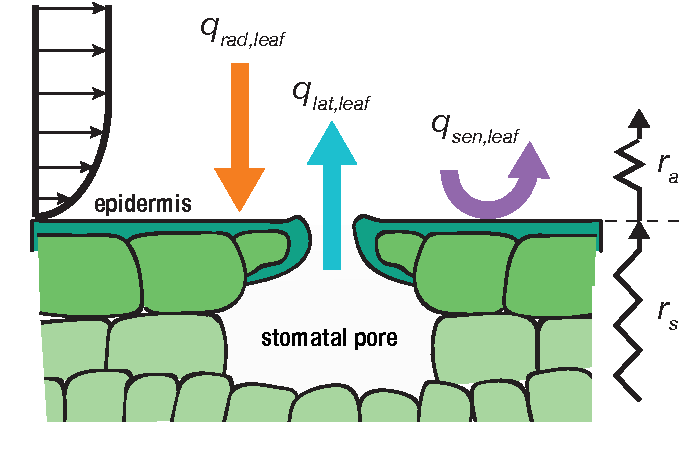
\includegraphics[width=0.8\textwidth]{\figdir/leafsurface-crop.pdf}
	\caption{Schematic representation of leaf surface with energy balance as given by \cref{eq:energybalance}. The radiative flux $q_{\mathit{rad,leaf}}$  absorbed by the leaf is balanced by the sensible $q_{\mathit{sen,leaf}}$ and the latent heat flux $q_{\mathit{lat,leaf}}$ leaving the leaf surface. The stomatal resistance 
	$r_s$ influences the latent heat flux and the aerodynamic resistance $r_a$ influences both the sensible and the latent heat fluxes. }
	\label{fig:leaf_energybalance}
	\end{figure}

The stationary energy balance is given as:
\begin{equation}
{q_{\mathit{rad},\mathit{leaf}}} - {q_{\mathit{lat},\mathit{leaf}}} - {q_{\mathit{sen},\mathit{leaf}}} = 0
\label{eq:energybalance}
\end{equation}
where ${q_{\mathit{rad},\mathit{leaf}}}$ (W\,m$^{-2}$) is the radiative flux, ${q_{\mathit{sen},\mathit{leaf}}}$ (W\,m$^{-2}$) is the sensible heat flux and ${q_{\mathit{lat},\mathit{leaf}}}$ (W\,m$^{-2}$) is the latent heat flux \citep{Majdoubi2009, Bruse1998, Dauzat2001,Hiraoka2005}. Positive sensible and latent heat fluxes are defined as heat transfer from the leaf into the air. The sensible heat flux due to convective heat transfer from leaf surface to the air is given as:
\begin{equation}
{q_{\mathit{sen,leaf}}} = {h_{c,h}} \left( {{T_{\mathit{leaf}}} - T} \right) = \frac{{2\rho {c_p}}}{{{r_a}}} \left( {{T_{\mathit{leaf}}} - T} \right)
\label{eq:sensibleheatflux}
\end{equation}
where $h_{c,h}$ (W\,m$^{-2}$\,K$^{-1}$] is the convective heat transfer coefficient (CHTC), $T_{\mathit{leaf}}$ (K) is the leaf surface temperature, $T$ (K) is the air temperature and $r_a$ (s\,m$^{-1}$) is the aerodynamic resistance of the boundary layer around the leaf. A factor 2 is present in the equation as the sensible heat flux occurs on both sides of the leaf. The aerodynamic resistance $r_a$ (s\,m$^{-1}$) is given as \citep{Dauzat2001, Robitu2006}:
\begin{equation}
{r_a} = C\;{\left( {\frac{l}{{\left| {\bar u} \right|}}} \right)^{1/2}}
\label{eq:ra}
\end{equation}
where $C=130$ s$^{0.5}$\,m$^{-1}$ is the proportionality factor and $l$ (m) is the characteristic leaf size ranging from 0.02 m for conifers and up to 0.5 m for tropical plants \citep{Bruse1998}. The latent heat flux from leaf to air due to transpiration is defined as:
\begin{equation}
{q_{lat,leaf}} = {L_v} \, {g_{v,leaf}}
\label{eq:latentheatflux}
\end{equation}
where $L_v=\num{2.5e6}$ J kg$^{-1}$ is latent heat of vaporization. The water vapor mass flux $g_{\mathit{v,leaf}}$ from leaf into the air is given as:
\begin{equation}
{g_{\mathit{v,leaf}}} = {h_{c,m}}\left( {{p_{\mathit{v,leaf}}} - {p_v}} \right) = \frac{{\rho {R_a}}}{{p{R_v}}} \, \frac{1}{{{r_a} + {r_s}}}\left( {{p_{\mathit{v,leaf}}} - {p_v}} \right)
\label{eq:vapourflux}
\end{equation}
where $h_{c,m}$ (s\,m$^{-1}$) is the convective mass transfer coefficient (CMTC), $p_{\mathit{v,leaf}}$ [Pa] is the vapor pressure at the leaf, $p_v$ (Pa) is the vapor pressure of the air above the leaf boundary layer, $r_s$ (s\,m$^{-1}$) is the stomatal resistance and $R_a=287.042$ J\,kg$^{-1}$\,K$^{-1}$ and $R_v=\num{461.524}$ J kg$^{-1}$~K$^{-1}$ are the gas constants of dry air and water vapor, respectively. In the present study, we assume that there is no condensation or rain on the leaf surface and so evapotranspiration is only due to transpiration through the leaf stomata. Therefore, the vapor pressure at the leaf is the vapour pressure within the leaf stomata which is close to the saturation vapor pressure at the leaf temperature, thereby we can assume
\begin{equation}
p_{\mathit{v,leaf}}=p_{\mathit{vsat,stom}} \left(T_{\mathit{leaf}}\right)
\end{equation}

The additional resistance $r_s$ is due to the stomatal regulatory control of the leaf. In the present study, the stomatal resistance is modeled as a function of climatic conditions: $q_{\mathit{r,sw}}$ the short-wave radiative flux in the air and $D$ (kPa) the vapor pressure deficit in the air, the difference between the saturation vapor pressure and the vapor pressure of the air
\begin{equation}
D \equiv p_{\mathit{v,sat}} - p_v
\end{equation}

The stomatal resistance is given as:
\begin{equation}
{r_s} = {r_{s,{\mathit{min}}}}{f_1}({q_{r,}}_{sw}){f_2}(D)
\label{eq:rs}
\end{equation}
where $r_{\mathit{s,min}}$ (s\,m$^{-1}$) is the minimal stomatal resistance and
\begin{align}
f_1 &= \frac{a_1 + q_{\mathit{r,sw}}}{a_1 + q_{\mathit{r,sw}}}\\
f_2 &= 1 + a_3 (D-D_0)^2
\end{align}
are multiplicative functions describing the stomatal resistance change due to short-wave radiation and vapor pressure deficit in the air, respectively. The constants of the empirical functions are $a_1=169$ W\,m$^{-2}$, $a_2=18$ W~m$^{-2}$, $a_3=\num{0.005}$ kPa$^{-2}$ and $D_0=1.2$ kPa \citep{Kichah2012}. The minimum stomatal resistance $r_{s,\mathit{min}}$, the resistance when the stomata are fully open, depends on the plant type: e.g. $150$ s~m$^{-1}$ for impatiens, $200$ s~m$^{-1}$ for grass, $400$ s\,m$^{-1}$ for gloxinia and deciduous plants \citep{Baille1994, Bruse1998}. It must be noted that various other models exist in literature for the stomatal resistance and an overview is given by \cite{Damour2010}. The present model is chosen as it is a simple model which can be used to consider the influence of environmental conditions. The energy balance (\cref{eq:energybalance}) is solved once the leaf surface temperature $T_{\mathit{leaf}}$ is known. Combining \cref{eq:energybalance,eq:sensibleheatflux,eq:latentheatflux}, the leaf temperature is given as:
\begin{equation}
{T_{\mathit{leaf}}} = T + \frac{{{q_{\mathit{rad,leaf}}} - {q_{\mathit{lat,leaf}}}}}{{{h_{c,h}}}}
\label{eq:solveleaft}
\end{equation}
where the equation is solved iteratively as $q_{\mathit{lat,leaf}}$ is dependent on the leaf temperature.

\section{Radiation within vegetation}
\label{sec:vegradiation}

The net radiative flux field $q_r$ (W\,m$^{-2}$) in the air domain is the sum of short-wave and long-wave radiative fluxes:
\begin{equation}
{q_r} = {q_{\mathit{r,sw}}} + {q_{\mathit{r,lw}}}
\label{eq:rad1}
\end{equation}
where $q_{\mathit{r,sw}}$ (W\,m$^{-2}$) is the short-wave radiative flux and $q_{\mathit{r,lw}}$ (W\,m$^{-2}$) is the long-wave radiative flux. The source or sink of the radiative flux in the air is equal to the divergence of the net radiative flux:
\begin{equation}
s_{q,r} = \nabla \cdot q_r
\label{eq:rad2}
\end{equation}
and is due to the absorption and emission of radiation by the equivalent leaf area of the vegetation:
\begin{equation}
{s_{q,r}} = a \, {q_{\mathit{rad,leaf}}}
\label{eq:rad3}
\end{equation}
where $q_{\mathit{rad,leaf}}$ (W\,m$^{-2}$) is the net radiative flux at the leaf surface. Substituting \cref{eq:rad1,eq:rad2} into \cref{eq:rad3}, we can determine the net radiative flux absorbed by the leaf:
\begin{equation}
{q_{\mathit{rad,leaf}}} = \frac{{\nabla  \cdot {q_{\mathit{r,sw}}} + \nabla  \cdot {q_{\mathit{r,lw}}}}}{a}
\label{eq:qradleaf}
\end{equation}

In this study, we simplify the formulation of radiation within vegetation according to the studies of plants in greenhouses \citep{Boulard2002, Majdoubi2009, Fatnassi2006, Kichah2012}. The approach employs a simplified empirical formulation of radiation distribution within vegetation. The advantage of this approach is that radiation within vegetation can be determined with a very low computational expense while providing sufficient accuracy. Such an approach is ideal for a parametric study on the dominant factors driving the transpirative cooling effect of vegetation. However, the downside of the model is that the long-wave radiation exchanges between surroundings cannot be evaluated.

The short-wave radiative flux $q_{\mathit{r,sw}}$ within a vegetation volume is determined using Beer-Lambert law:
\begin{equation}
{q_{r,sw}}(z) = {q_{r,sw,0}}\,{\exp}\left\{ - \beta \int_z^H {a\left( z \right)} \;\mathrm{d}z \right\}
\label{eq:beerlambert}
\end{equation}

where $q_{r,sw,0}$ (W\,m$^{-2}$) is the short-wave radiative flux hitting the top of the vegetation and $\beta=0.78$ is the extinction coefficient for short-wave radiation. The integral defines the net density of leaves that is present from the top of the vegetation canopy to the height where the short-wave radiative flux is evaluated. The simplification we consider in this study is that the sun is positioned directly above vegetation, i.e. mid-day condition with a solar altitude $\phi=90^{\circ}$. A model with varying solar conditions is part of future research. The long-wave radiative flux is modelled empirically, as a function of the downward long-wave radiative flux, i.e. from the sky. It is given by:
\begin{equation}
\nabla  \cdot {q_{\mathit{r,lw}}} = {C_{\mathit{lw}}}\frac{{{q_{\mathit{r,lw,} \downarrow }}}}{H}
\end{equation}
where $C_{lw}=0.04$ is an empirical constant for quantifying the net absorption of long-wave radiation \citep{Kichah2012}. Using this approach, the thermal emission of the leaves can be empirically modeled. The downward long-wave radiative flux is taken to be the long-wave radiative flux from sky, i.e. ${q_{\mathit{r,lw,} \downarrow }}$ with a sky temperature of $T_{\mathit{sky}}=15$ $^{\circ}$C \citep{Saneinejad2014}.

\section{Numerical model}

The vegetation model, described in \cref{sec:cons_incompressible,sec:sourceterms,sec:leafenergy,sec:vegradiation}, is implemented into the OpenFOAM finite volume solver \citep{Weller1998a}. The steady-state velocity field is solved using the SIMPLE pressure-velocity coupling algorithm. A second-order central difference scheme is used for the gradient operator and a second-order linear upwind differencing scheme for the convective terms. The convergence criterion for the residuals is set to $10^{-8}$ based on sensitivity analysis. The computational domain size and the numerical scheme are chosen based on CFD best practices \citep{Blocken2015, Franke2007, Tominaga2008}.

\subsection{Simulation domain}
The simulation of single row of trees is represented by a 2D porous domain ($x\times z$ axis) consisting of a $1\times1$ m$^2$ ($x\times z$ axis) porous vegetation region as shown in \cref{fig:domain}, while infinitely long in the y-direction, where the source terms (\crefrange{eq:source_density}{eq:source_eps}) are non-zero. The computational domain is $35\times11.5$ m$^2$ ($x\times z$ axis) and the mesh resolution is determined by performing a grid sensitivity analysis. The domain is discretized into a regular grid with \num{40000} rectangular cuboidal cells. The smallest cell is at the edge of the tree row ($\Delta x = \Delta z = 0.01$ m) and the expansion ratio to the outflow, inlet, ground and top boundaries are 1.05, 1.05, 1.05, and 1.15, respectively. 

	\begin{figure}[h]
	\centering
	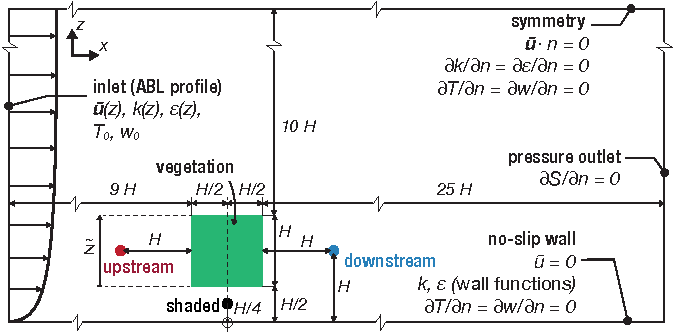
\includegraphics[width=\textwidth]{\figdir/domain-crop.pdf}
	\caption{Simulation domain of the reference case with $H=1$ m with description of the domain and the boundary conditions. The porous vegetation region is indicated in green ({\color{flatuidarkgreen}$\blacksquare$}) where leaf area density $a=10$ m$^2$\,m$^{-3}$ and zero everywhere else. The red point ({\color{flatuidarkred}$\bullet$}) indicate the upstream $(x=-1.5H,y=H)$, blue ({\color{flatuidarkblue}$\bullet$}) indicate the downstream $(x=1.5H,y=H)$, and black ($\bullet$) indicate the shaded $(x=0,y=H/4)$ data sampling location.}
	\label{fig:domain}
	\end{figure}

The environmental factors that are varied for the parametric study are wind speed, ambient air temperature, relative humidity (RH) and solar radiation intensity. The environmental factors are tabulated in \cref{tab:environmentalcond}.  Similarly, the properties of the vegetation are tabulated in cref{tab:plantcond} and the parameters that are varied are leaf area density, stomatal resistance, leaf size, tree height and number of tree rows, which are presumed to have an influence on the transpirative cooling effect of vegetation. The upper and lower bounds of the parameters are chosen based on values from literature. The reference tree is chosen to be a densely foliated garden hedgerow in a midday conditions. 


\ctable[
caption = {Environmental factors varied in the parametric study},
label   = {tab:environmentalcond},
pos = t,
mincapwidth = \textwidth,
]{lrr}{}{
	\FL
	Parameter 									& Range & Reference 	
	\ML
	Solar radiation, $q_{\mathit{r,sw,0}}$  			& $[100, 400, 800, 1000]$ & $800$	 \\
	Wind speed, $U_{\mathit{ref}}$ 						& $[0.1,0.25,0.5,0.75,1,2,3,5]$  & $1$	\\
	Air temperature, $T_0$   							& $[20, 30]$ & $30$	\\
	Relative humidity, $\textit{RH}$   					& $[20, 30, 40, 50, 60, 70, 80]$ 	& $60$	
	\LL}

\ctable[
caption = {Plant properties varied in the parametric study},
label   = {tab:plantcond},
pos = t,
mincapwidth = \textwidth,
]{lrr}{}{
	\FL
	Parameter 									& Range 	& Reference 
	\ML
	Leaf area density, $a$  							& $[1, 3, 5, 7, 10]$  	& $10$\\
	Wind speed, $r_{\mathit{s,min}}$  					& $[50, 100, 125, 150, 175, 200, 250, 300]$& $150$	 \\
	Leaf size, $l$   										& $[0.01, 0.05, 0.1, 0.2, 0.3, 0.4]$ & $0.1$\\
	Tree height , $n\,H$   								& $[1, 2, 3, 5, 10]$ & $1$		 \\
	$\mathcal{N}^{\underline{o}}$\, of tree rows, $n$   						& $[1, 2, 5, 10]$ & $1$	
	\LL}



\subsection{	Boundary conditions}

An atmospheric boundary layer (ABL) profile is prescribed at the inlet \citep{Richards1993}:
\begin{align}
\tavg{u}(z) &= \frac{{{u_*}}}{\kappa }{\text{ln}}\left( {\frac{{z + {z_0}}}{{{z_0}}}} \right) \\
k &= \frac{{{u_*}^2}}{{\sqrt {{C_\mu }} }} \\
\varepsilon  &= \frac{{u_*^3}}{{\kappa \left( {z + {z_0}} \right)}}
\end{align}

where $\tavg{u}(z)$ (m\,s$^{-1}$) is the horizontal inlet velocity at height $z$, $u_*$ (m\,s$^{-1}$) is the friction velocity, $\kappa=0.41$ is von K\'arm\'an constant, $z_0=\num{0.0217}$ m is the aerodynamic roughness height and $C_{\mu}=0.09$. The inlet boundary conditions for air temperature $T$ and humidity ratio $w$ are for simplicity uniform profiles, $T(z)=T_0$ and $w(z)=w_0$ and varied individually during the parametric study as tabulated in \cref{tab:environmentalcond}.

The ground is modeled using standard wall functions and is considered to be adiabatic. This ensures that the thermal influence of the ground is not present when measuring the cooling effect of vegetation on air. Even though, in reality, the thermal influence of the ground on the air temperature is an important factor, in the present study this simplification was chosen to isolate the influence of transpirative cooling of vegetation. A zero normal gradient boundary condition is applied for the humidity ratio. At the top, a slip velocity boundary condition is used and the temperature and humidity ratio are prescribed a zero normal gradient boundary condition. The outlet of the domain is set to a pressure outlet. The boundary conditions for T and w at outlet are zero normal gradient boundary conditions. 

\subsection{Numerical solution procedure}

In the present study, the following strategy is used for solving the coupled vegetation-air problem:

\begin{enumerate}
\item Solve the energy balance at the leaf surface:
\begin{enumerate}
	\item Determine the radiative flux $q_{\mathit{rad,leaf}}$ using \cref{eq:qradleaf}.
	\item Calculate the stomatal and aerodynamic resistances $r_a$ and $r_s$ using \cref{eq:ra} and \cref{eq:rs}, respectively.
	\item Perform an initial estimate of leaf temperature $T_{\mathit{leaf}}=T$.
	\item Calculate the saturated vapor pressure at the leaf surface $p_{\mathit{vsat,leaf}}=f(T_{\mathit{leaf}})$.
	\item Calculate the latent heat flux $q_{\mathit{lat,leaf}}$ using \cref{eq:latentheatflux}. 
	\item Correct the leaf temperature $T_{\mathit{leaf}}$ using \cref{eq:solveleaft}.
	\item Repeat steps (d) to (f) until the leaf temperature has converged with a convergence criterion of \num{e-8}.
\end{enumerate}
\item Calculate all vegetation source terms $s_\rho$, $s_u$, $s_T$, $s_w$, $s_k$ and $s_{\varepsilon}$ using Eqs. \cref{eq:source_density,eq:source_mom,eq:source_temp,eq:source_humi,eq:source_k,eq:source_eps}.
\item Solve for the steady-state flow field, \crefrange{eq:conservationeq_incompressible1}{eq:conservationeq_incompressible6}.
\item Repeat steps (1) to (3) until residuals of \crefrange{eq:conservationeq_incompressible1}{eq:conservationeq_incompressible6} have reached the convergence limit of \num{e-8}.
\end{enumerate}

The algorithm of the vegetation model is implemented as an OpenFOAM C++ library. To satisfy the energy balance problem, the leaf temperature is determined iteratively using \cref{eq:solveleaft}, with the air temperature as an initial guess for leaf temperature. The energy balance is satisfied once the leaf temperature converges. The numerical model is validated and is used thereafter to investigate the influence of environmental factors and tree properties on the transpirative cooling effect.

\section{Validation of vegetation model}

The vegetation model is first validated against the numerical and experiment study of \cite{Kichah2012}. The study provides measurement and numerical (CFD) results of flow through impatiens (jewelweed) plants in a greenhouse. The study investigates the heat and moisture exchanges between vegetation and the air and provides a comprehensive dataset of the response of vegetation to environmental conditions. The simulation domain is adapted according to the study, where the impatiens plants are placed on a table, \cref{fig:domain_validation}.

	\begin{figure}[h]
		\centering
		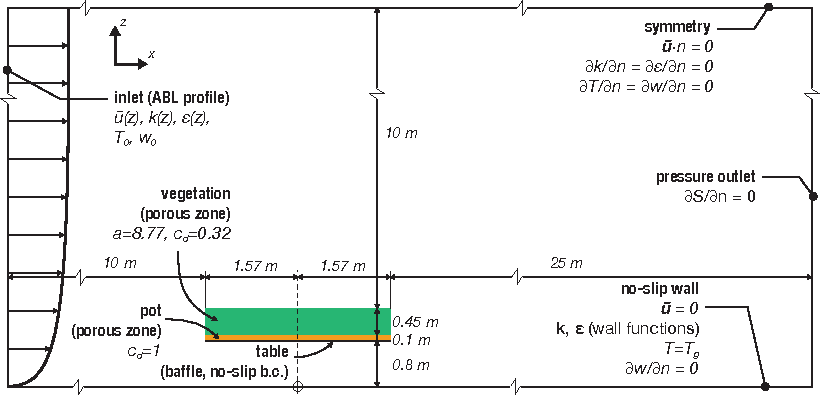
\includegraphics[width=\textwidth]{\figdir/domain_validation-crop.pdf}
		\caption{Simulation domain and boundary conditions for the validation case \cite{Kichah2012}. The impatiens plant in indicated in green ({\color{flatuidarkgreen}$\blacksquare$}) and plant plot in orange ({\color{flatuiorange}$\blacksquare$}). Both are regions are modeled as porous zone with drag coefficients $c_d=0.32$ and $c_d=1$, respectively. The boundary conditions of the simulation are tabulated in \cref{tab:validationparameters} and correspond to 14:00 on June 15$^{\mathrm{th}}$, 2009.}
		\label{fig:domain_validation}
	\end{figure}

The plants and the pots are both modeled as porous medium with different drag coefficients. The drag coefficient of the plant and pot are $c_d=0.32$ and $c_d=1$, respectively. The table is modeled as an internal wall (i.e. baffle) that enforces a standard wall boundary condition. The boundary condition of the ground is $T=T_g$ and standard wall functions are used. The top boundary is a symmetry plane. The outlet is taken to be far enough to ensure zero-normal gradient for all variables and a zero pressure is imposed. The inlet boundary conditions are tabulated in \cref{tab:validationparameters}, corresponding to a greenhouse in a sunny day on 15$^{\mathrm{th}}$ July 2009 at 14:00. Based on a mesh sensitivity analysis, a regular grid discretization is chosen with smallest cells at the edge of the vegetation ($\Delta x=0.01,\,\Delta y=\num{0.0055}$) and a total number of cells of \num{24000}. The grid expansion ratio from the vegetation edges to the outflow, inlet, ground and top boundaries are $1.05$, $1.11$, $1.13$ and $1.15$, respectively. 

	\begin{figure}[h]
	\centering
	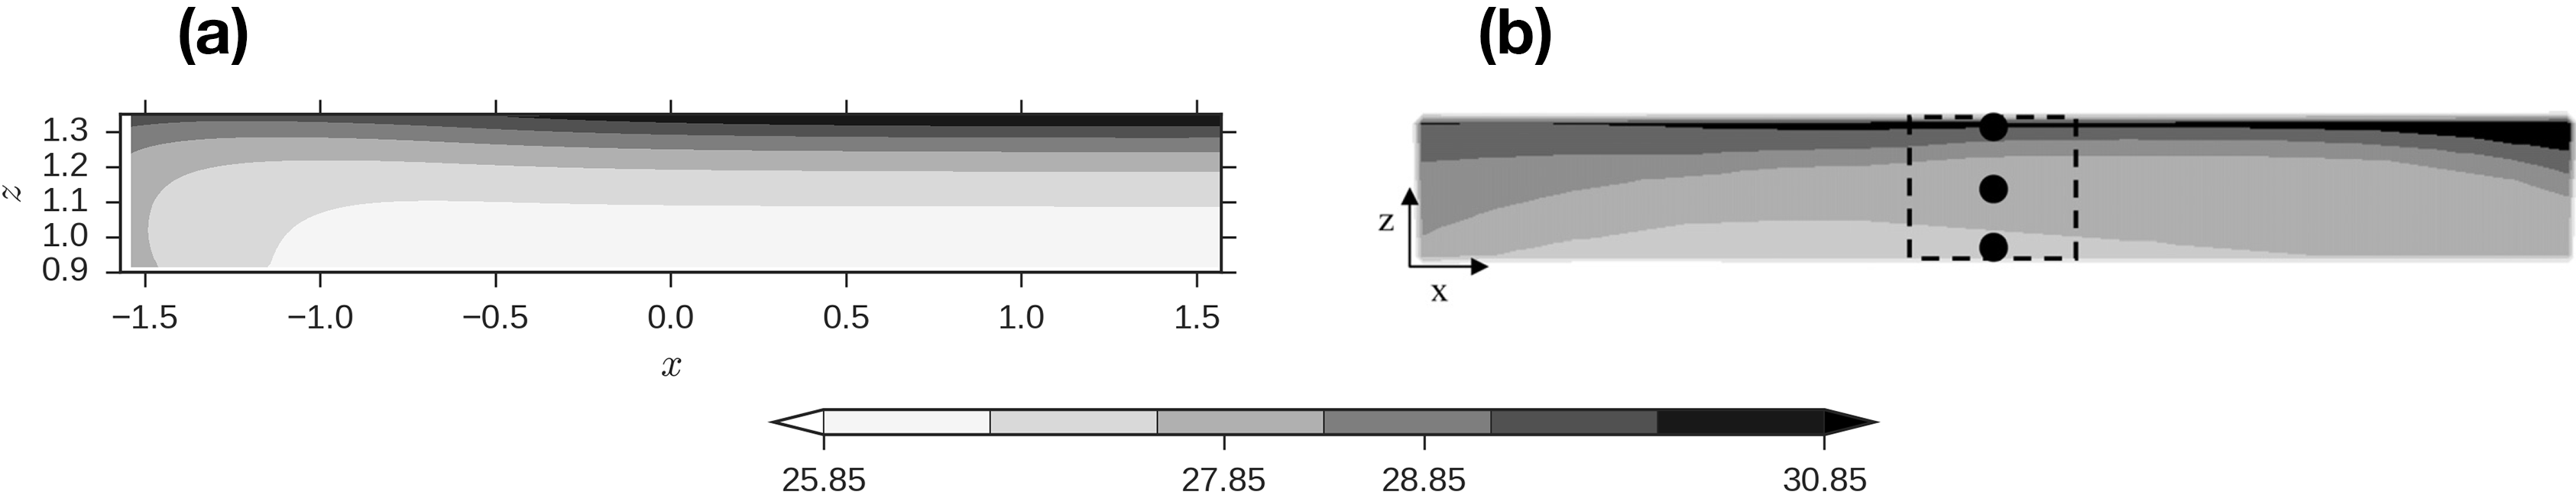
\includegraphics[width=\textwidth]{\figdir/comparions_TL_updated.png}
	\caption{Comparison of leaf temperature $T_\mathit{leaf}$ ($^{\circ}$C) within vegetation ($-1.5\le x \le 1.5$) and ($0.9 \le z \le 1.35$): \subfig{a} present study and \subfig{b} numerical simulation results from \citep{Kichah2012}. The three dots (\textit{bottom}: $z=0.9$ m, \textit{middle}: $z=1.125$ m and \textit{top}: $z=1.35$ m) indicate the temperature probe positions, \cref{tab:comparisonT}.}
	\label{fig:comparions_TL_updated}
	\end{figure}

\cref{fig:comparions_TL_updated} shows the leaf temperature $T_{\mathit{leaf}}$ distribution of the vegetation and is compared with numerical results from the original study \citep{Kichah2012}. We see that the temperature ranges (between $25$ $^{\circ}$C and $31$ $^{\circ}$C) are in good agreement. However, the leaf temperature contours are different between the two simulations. The general trend in vertical temperature distribution is in agreement, with peak temperatures appearing close to the top of the vegetation due to radiation absorption. The difference observed between the present model and \cite{Kichah2012} could be due to the use of a turbulence model as the turbulence production and dissipation due to vegetation (Eqs. (11) and (12)) is not done in \cite{Kichah2012}. However, it is shown by \cite{Sanz2003} that the influence of vegetation on turbulence has to be modeled to ensure physically accurate turbulence characteristics. Moreover, we employ the realizable $k-\varepsilon$ turbulence closure in contrast to the standard $k-\varepsilon$ used by \cite{Kichah2012}. The realizable $k-\varepsilon$ model is chosen as it provides more accurate wake characteristics leeward of a porous medium \citep{Santiago2007, Shih1995}. The choice of turbulence model is known to have an impact on parameters such as recirculation length \citep{Santiago2007} and this could result in some difference in the leaf temperature contours. 

\ctable[
caption = {Environmental conditions used in \cite{Kichah2012}. Data obtained for condition at 14:00 on June 15$^{\mathrm{th}}$, 2009.},
label   = {tab:validationparameters},
pos = b,
mincapwidth = \textwidth,
]{lr}{}{
	\FL
	Parameter 									& Value
	\ML
	Air temperature, $T_0$  					& $32$ $^{\circ}$C\\
	Ground temperature $T_g$					& $24$ $^{\circ}$C\\
	Humidity ratio $w_0$  						& $6.21$ g\,kg$^{-1}$\\
	Solar radiation, $q_{\mathit{r,sw,0}}$   	& $99$ W\,m$^{-2}$ \\
	Long-wave radiation, $q_{\mathit{r,lw},\downarrow}$	& $522$ W\,m$^{-2}$
	\LL}

Furthermore, the validation is performed by comparing the leaf and air temperatures with the numerical and experimental results from \cite{Kichah2012}. The numerical and experimental values of leaf temperature $T_{\mathit{leaf}}$ values are obtained for three positions: ``\textit{bottom}'' $(x=0,\,z=0.9)$, ``\textit{middle}'' $(x=0,\,z=1.125)$ and ``\textit{top}'' $(x=0,\,z=1.35)$. The numerical and experimental values of the air temperature $T_{\mathit{leaf}}$ at position ``\textit{middle}'' are also compared, as shown in \cref{tab:comparisonT}. The comparison shows that the numerical results from the present study are in better agreement with the experiments than the numerical results of \cite{Kichah2012}. At the top of the vegetation, the difference between the numerical and experimental results are the highest with $T^{\mathit{num}}-T^{\mathit{exp}}=1.0$ $^{\circ}$C for both the present study and  \cite{Kichah2012}. The deviation on the top between the predicted and the measured temperatures could be due to the simplification in the leaf distribution. The numerical models assume the leaf area density to be homogeneously distributed, however, in reality, it varies in height. This influences the radiation absorption within vegetation and will impact the heat and mass exchanges. Generally, the leaf temperature trend is seen to be slightly overestimated and the air temperature to be slightly underestimated. However, as the deviation is only within $1.0$ $^{\circ}$C, we consider the predicted results to be sufficiently accurate.  

\ctable[
caption = {Comparison of leaf temperature $T_{\mathit{leaf}}$ at various heights and air temperature $T$ in the middle of vegetation. Experimental and numerical data obtained from \citep{Kichah2012}.},
label   = {tab:comparisonT},
pos = p,
mincapwidth = \textwidth,
sideways,
]{lrrrrr}{}{
	\FL
	\multirow{2}{*}{Parameter} 					& \multirow{2}{0.25\linewidth}{Experimental \citep{Kichah2012}} 	& \multicolumn{2}{c}{Numerical} & \multicolumn{2}{c}{$T^{\mathit{num}}-T^{\mathit{exp}}$} \\
												& 						& \citep{Kichah2012} & Present & \citep{Kichah2012} & $T^{\mathit{present}}-T^{\mathit{exp}}$
	\ML
							 &  &  &  & & \\ 
	\multicolumn{6}{l}{Leaf temperature $T_{\mathit{leaf}}$ ($^{\circ}$C)} \\

	\hspace{2em}\textit{top} ($z = 1.35$ m) & $29.5$ & $30.5$ & $30.5$ & $1.0$ & $1.0$\\ 
	\hspace{2em}\textit{middle} ($z = 1.125$ m) & $26.7$ & $28.0$ & $27.0$ & $1.3$ & $0.3$\\ 	
	\hspace{2em}\textit{bottom} ($z = 0.9$ m) & $26.1$ & $27.6$ & $26.2$ & $1.5$ & $0.1$\\ 
								 &  &  &  & & \\ 
	\multicolumn{6}{l}{Air temperature $T$ ($^{\circ}$C)} \\	
	\hspace{2em}\textit{middle} ($z = 1.125$ m) & $28.11$ & $28.5$ & $27.9$ & $-0.4$ & $-0.2$ \\
	
	\LL}


\section{Impact of row of trees on the microclimate}

The developed numerical model is first used to understand the impact of a single row of trees on the surrounding microclimate. The transpirative cooling effect of vegetation is determined as the change in the Universal Thermal Climate Index (\textit{UTCI}). Thereafter, a parametric study is performed to determine the impact of different environmental factors, tree properties and vegetation. The simulation domain described in \cref{fig:domain} is used as the reference case for the parametric study. The environmental boundary conditions are given in \cref{tab:environmentalcond} and the tree properties are tabulated in \cref{tab:plantcond}. To ensure fair comparison in the parametric study, the stomatal resistance is fixed to the minimum stomatal resistance $r_s=r_{\textit{s,min}}$ and is assumed to be independent of the radiation and humidity levels of the environment. The influence of the stomatal model is investigated separately. As mentioned above, the study assumes that the ground is adiabatic to isolate the influence of transpirative cooling effect of the tree row on the air. To study the impact of a single row of trees on the microclimate, the energy balance at the leaf surface and its implication on the flow field are studied first.

\subsection{Impact on energy balance at the leaf surface}

The energy balance at the leaf surface is defined by \cref{eq:energybalance}, where the absorbed radiative heat flux is converted into latent and sensible heat fluxes. The average radiative flux into the leaf is $\langle q_{\textit{rad,leaf}} \rangle =77$ W\,m$^{-2}$ for both cases. In the case of constant stomatal resistance, $r_s=r_{\textit{s,min}}$, the average sensible flux is $\langle q_{\textit{sen,leaf}} \rangle = -50$ W\,m$^{-2}$ (negative sign indicates cooling of the air) and the average latent heat flux is $\langle q_{\textit{lat,leaf}} \rangle =127$ W\,m$^{-2}$ used to evaporate water. In the case of varying stomatal resistance \cref{eq:rs}, the average sensible and latent heat fluxes are $9$ W\,m$^{-2}$ and $68$ W\,m$^{-2}$, respectively. To better understand how the radiative heat is converted, the heat flux distribution and the leaf temperature distribution within the foliage are studied. \cref{fig:profiles} shows the vertical distribution of heat fluxes and temperature along the vertical centre line within the centre of the foliage. \cref{fig:profiles}a shows that the heat fluxes are maximum at the top of the trees, where solar radiation is mostly absorbed due to the high density of vegetation with $a=10$ m$^2$\,m$^{-3}$. A high absorbed radiative heat results in a positive sensible heat flux (indicating heat is leaving the leaf and entering air) leading to an increase of the air temperature, as seen in \cref{fig:profiles}b. The latent heat flux is also positive due to transpiration at the leaf, \cref{eq:latentheatflux}. At lower heights, the radiation decays exponentially given the prior absorption of the short-wave radiation, \cref{eq:beerlambert}, resulting also in an exponential decay of the latent and sensible heat fluxes. At the bottom of the foliage, the sensible heat flux is negative as the radiation is low but transpiration still occurs, leading to cooling of the air. 

	\begin{figure}[t]
	\centering
	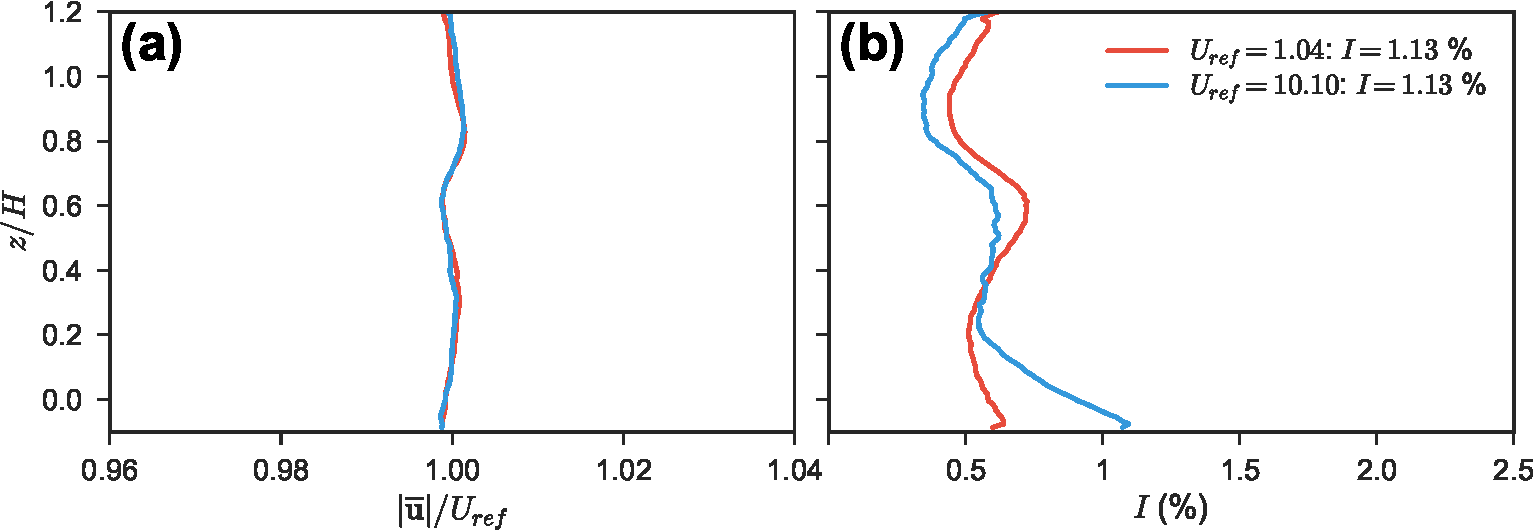
\includegraphics[width=\textwidth]{\figdir/profiles-crop.pdf}
	\caption{Vertical distribution at centre-line of the tree row with height  $\tilde{z}=0$ at bottom of the vegetation volume and  $\tilde{z}=1$ at top of the trees: \subfig{a} heat fluxes at the leaf surface (\cref{eq:energybalance}) and \subfig{b} temperature profiles of leaf temperature $T_{\textit{leaf}}$ ($^{\circ}$C) and air temperature $T$ ($^{\circ}$C).}
	\label{fig:profiles}
	\end{figure}

In the case of environmentally dependent stomatal resistance, the stomatal resistance is higher than minimum stomatal resistance, when the stomata are fully open. As stomatal resistance is inversely proportional to incident short-wave radiation (\cref{eq:rs}), this resistance is low at the top of the trees and high at the bottom of the trees. A higher stomatal resistance means that the CMTC is lower (\cref{eq:vapourflux}) and so the water vapor mass flux due to transpiration reduces. The reduced transpiration leads to higher leaf temperature and therefore lower cooling of the air provided by vegetation (\cref{fig:profiles}). With a minimum stomatal resistance, the average air temperature is $29.6$ $^{\circ}$C. Whereas, with higher stomatal resistances, the transpiration is reduced and the higher leaf temperature results in an average air temperature of $30.0$ $^{\circ}$C. To further understand the impact of stomatal resistance, the change in flow conditions due to vegetation is studied.

\subsection{Influence of vegetation on the flow field}

The heat, mass and momentum exchanges between the trees and the air determine the distribution of velocity, temperature and humidity. Furthermore, the turbulence intensity is increased due to the foliage. \cref{fig:flowfields}a shows the normalized velocity magnitude $\tavg{\mvec{u}}/U_{\textit{ref}}$, which shows the influence of momentum drag of the trees. The dashed box in the figure indicates the porous region where the source terms for vegetation are present. The figure shows that the wind speed is reduced by $50$\% behind the tree row. Furthermore, we see that the flow is slightly accelerated below the tree row between the tree bottom and the ground due to the blockage effect present in below a row of trees. \cref{fig:flowfields}b shows the increase in the turbulence intensity $\textit{TI}=(2/3\,k)/\tavg{\mvec{u}}$ due to the trees as it converts the mean kinetic energy into the turbulence kinetic energy. The TI inside the porous region is approximately $20$\% higher than the freestream flow. However, we see that the highest TI is observed in the wake region, $TI\approx50$\%, where the mean velocity is lowest and the TKE is high. Therefore, the impact of vegetation on the turbulence characteristics in a microclimate is not negligible. 

%	\begin{figure}[p]
%	\centering
%	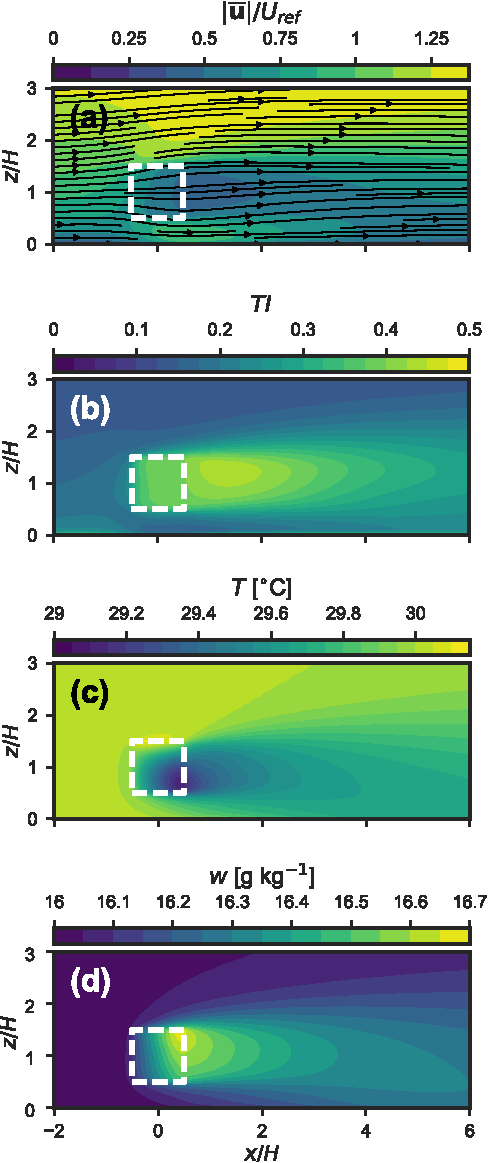
\includegraphics[height=0.9\textheight]{\figdir/flowfields_rearranged-crop.pdf}
%	\caption{Flow field past a single row of trees for the reference case with domain described in \cref{fig:domain}, with $r_s=r_{\textit{s,min}}$ and environmental and tree properties tabulated in \cref{tab:environmentalcond,tab:plantcond}, respectively. a) Normalized velocity $\tavg{\mvec{u}}/U_{\textit{ref}}$, b) turbulence intensity $\textit{TI}=(2/3~k)/\tavg{\mvec{u}}$ c) air temperature $T$ ($^{\circ}$C) and d) humidity ratio $w$ (g~kg$^{-1}$).}
%	\label{fig:flowfields}
%	\end{figure}

	\begin{sidewaysfigure}[p]
	\centering
	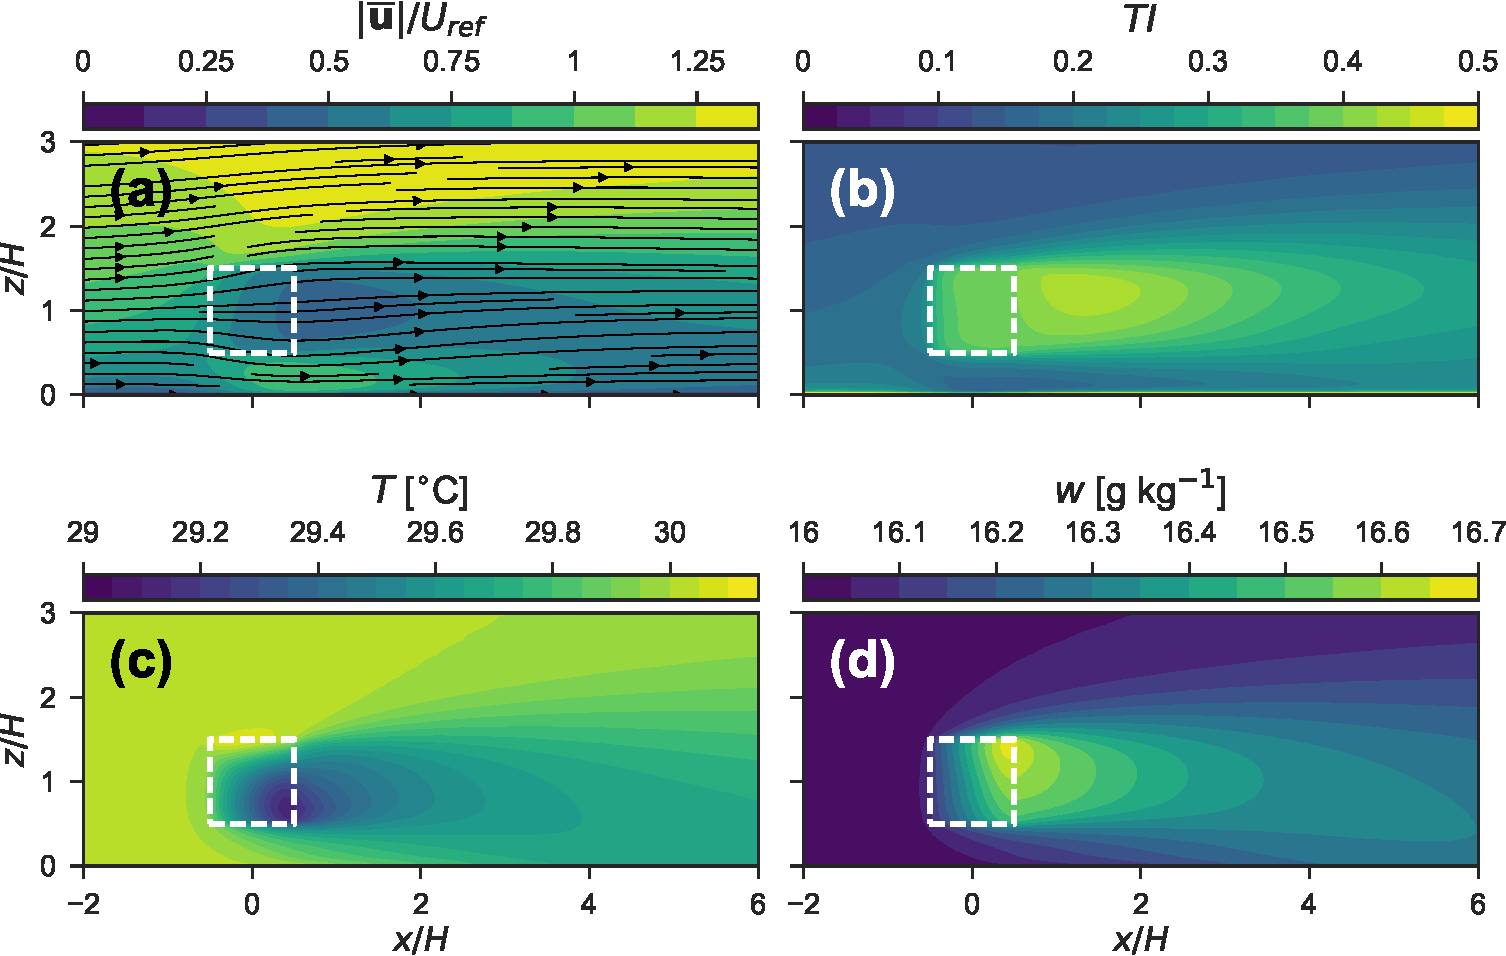
\includegraphics[width=\textwidth]{\figdir/flowfields-crop.pdf}
	\caption{Flow field past a single row of trees for the reference case with domain described in \cref{fig:domain}, with $r_s=r_{\textit{s,min}}$ and environmental and tree properties tabulated in \cref{tab:environmentalcond,tab:plantcond}, respectively. \subfig{a} Normalized velocity $\tavg{\mvec{u}}/U_{\textit{ref}}$, \subfig{b} turbulence intensity $\textit{TI}=(2/3\,k)/\tavg{\mvec{u}}$ \subfig{c} air temperature $T$ ($^{\circ}$C) and \subfig{d} humidity ratio $w$ (g\,kg$^{-1}$).}
	\label{fig:flowfields}
	\end{sidewaysfigure}

\cref{fig:flowfields}c shows the influence of a single row of trees on the air temperature. We observe that the highest cooling is at the bottom of the trees, where the absorbed radiation is lowest. The temperature is also lower towards the wake of the trees where the velocity is lower. Such ``\textit{oasis}'' effect of cool temperature region in the vicinity of vegetation has also been observed in various field measurements \citep{Kurn1994, Taha1997, Wong2003} and numerical studies \citep{Dimoudi2003,Gromke2011}. At the top of the tree foliage, we observe a higher air temperature due to higher absorption solar radiation but the temperature is only marginally higher than the ambient temperature. The air temperature increases because the leaf temperature is higher than the windward air temperature (\cref{fig:profiles}b). \cref{fig:flowfields}d shows that the humidity ratio increases and the highest humidity is at the top-downstream region of the trees. The figure shows that maximum transpiration occurs at the top of the trees, since solar radiation absorption is highest at the top of the trees and transpiration is also the process used by the trees to dissipate the absorbed radiative heat. The increase of humidity ratio towards the downstream region of the trees is due to the wind convecting the humidity towards the leeward side of the trees.

\subsection{Transpirative cooling effect of a row of trees}

A quantitative analysis of the transpirative cooling effect of a single row of trees and its impact on thermal comfort is possible by investigating the Universal Thermal Comfort Index (UTCI). The comfort index is expressed as an equivalent temperature and is determined from a human thermoregulatory response model coupled with a clothing model \citep{Fiala2001}. The equivalent temperature is dependent on the air temperature, humidity, wind speed and radiation and represents the temperature of a reference environment that would provide the same response for the reference person as it would in the actual environment. It is designed as an outdoor comfort index and is seen to outperform similar other comfort indices such as Perceived Temperature (PT), Physiological Equivalent Temperature (PET) and OUT\_SET* \citep{Jendritzky2012}. Furthermore, it can be used as an international standard for all assessments of the outdoor thermal conditions in various fields such as public weather services, public health systems and climate impact research. Therefore, the UTCI is used in this study to provide an indication of the comfort for a pedestrian in vicinity of trees. The UTCI is implemented in the BioKlima 2.6 software package and is calculated as ($^{\circ}$C):

\begin{equation}
UTCI = T + f \left(T,{T_{\textit{mrt}}},\left| \mvec{u}  \right|,RH\right)
\label{eq:UTCI}
\end{equation}

where it is a function of air temperature $T$, the mean radiant temperature $T_{\textit{mrt}}$, wind speed $|\mvec{u}|$ and relative humidity $RH$. The mean radiant temperature $T_{\textit{mrt}}$ is influenced by the long-wave and the short-wave radiation, which is a function of direct solar radiation $q_{\textit{r,sw}}$ and the solar altitude $\phi$. However, in this study we ignore the long-wave radiation component in the UTCI as the main goal of the study is to isolate the influence of transpirative cooling effect on the air and determine the influence of wind speed, temperature, RH, solar radiation and tree properties on the transpiration rate. By modeling the ground as an adiabatic surface, the soil heat storage could be decoupled from the interaction of transpirative cooling. We remark that, in the present study, diffuse solar radiation and long-wave radiation are not considered in the determination of mean radiant temperature for UTCI. These radiation components will be determined in future analysis for a more accurate assessment of pedestrian comfort, especially in the vicinity of buildings. The UTCI provides an indication of the thermal stress experienced by a pedestrian, as tabulated in \cref{tab:utcitable}. The UTCI values that lie between $18$ $^{\circ}$C and $26$ $^{\circ}$C comply as “\textit{thermal comfort zone}” \citep{Marshall1987}. A UTCI value in the range of a moderate heat stress (HS) level can result in sweating for the reference person after 30 minutes, where fatigue is possible after prolonged exposure or physical activity \citep{Blazejczyk2012,Bazejczyk2013}. A UTCI value in the range of a strong HS level results in an instantaneous change in skin temperature and introduces the risk for sunstroke and muscle cramp after prolonged exposure. A very strong HS level is considered dangerous showing increase in internal body temperature within 30 minutes with high possibility of sunstroke and muscle cramp after prolonged exposure. An extreme HS level is considered highly dangerous with high likeliness of heat stroke.

\ctable[
caption = {UTCI thermal heat stress categories \citep{Brode2012, Oke2017a}.},
label   = {tab:utcitable},
pos = p,
mincapwidth = \textwidth,
sideways,
]{rll}{}{
	\FL
	UTCI ($^{\circ}$C)									& Thermal stress categories  	& Physiological responses 
	\ML
	& & \\
	$> 46$							 					& Extreme heat stress (HS) 		& Increase in core temperature\\
														& 								& \\
	\numrange{38}{46}									& Very strong HS				& \multirow{2}{0.65\linewidth}{Small core to skin temperature gradient ($< 1$ K), Sweat rate increase ($> 650$ g\,h$^{-1}$ at limit) }\\
														& 								& \\
														& 								& \\
	\numrange{32}{38}									& Strong HS						& Sweat rate $> 200$ g\,h$^{-1}$\\
													 	& 								& \\
	\numrange{26}{32}									& Moderate HS					& Increased rate of sweating and skin temperature\\	
														& 								& \\
	\numrange{9}{26}									& No thermal stress				& Comfortable, sweat rate $< 100$ g\,h$^{-1}$ \\
	\LL}	


	
	\begin{figure}[p]
		\centering
		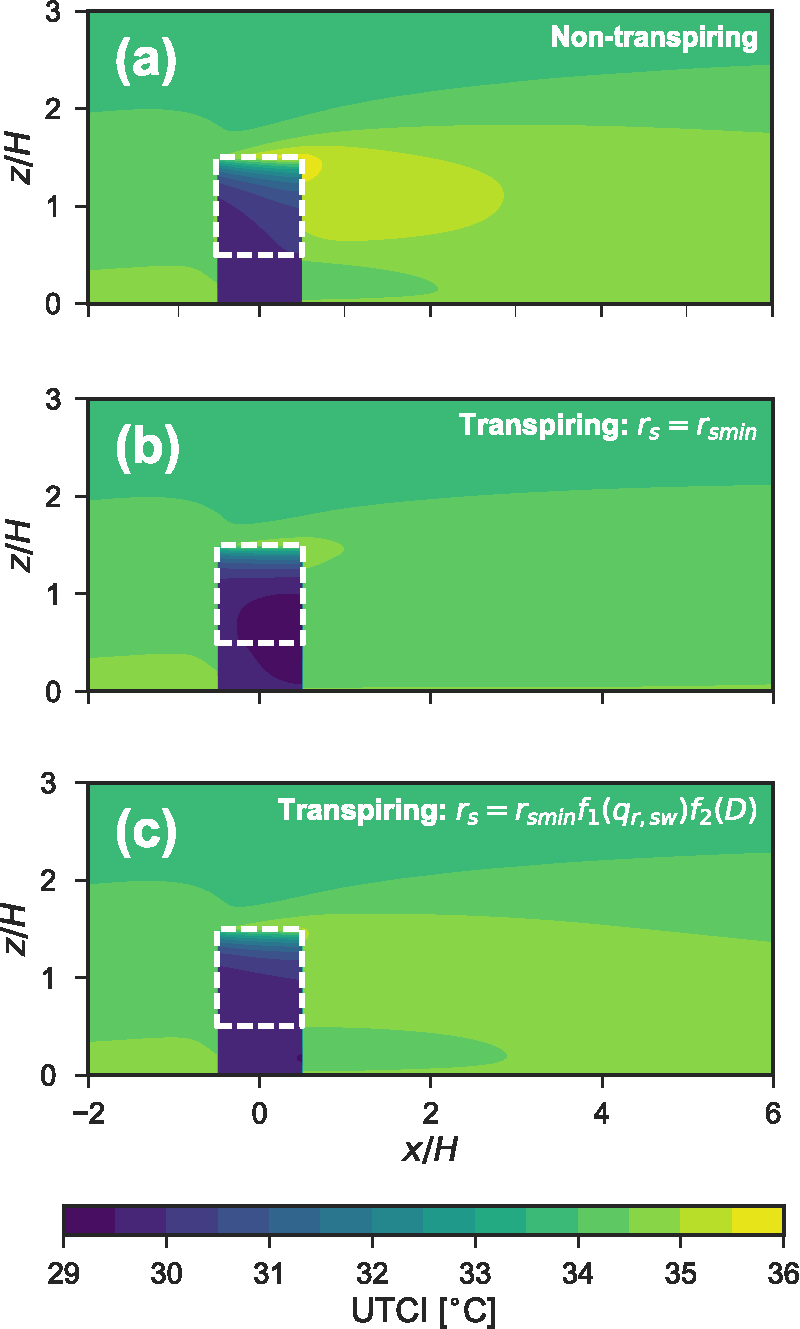
\includegraphics[height=0.8\textheight]{\figdir/utci_part1-crop.pdf}
		\caption{Transpirative cooling effect of a single row of trees. The influence of the trees on the Universal Thermal Comfort Index (UTCI) ($^{\circ}$C) for \subfig{a} in non-transpiring condition (NT); in transpiring condition (T) for \subfig{b} constant stomatal resistance, $r_{\textit{s,min}}$ and \subfig{c} for varying stomatal resistance $r_s=r_{\textit{s,min}} f(q_{\textit{r,sw}})f(D)$.}
		\label{fig:utcifield1}
	\end{figure}
	
	
	\begin{figure}[p]
		\centering
		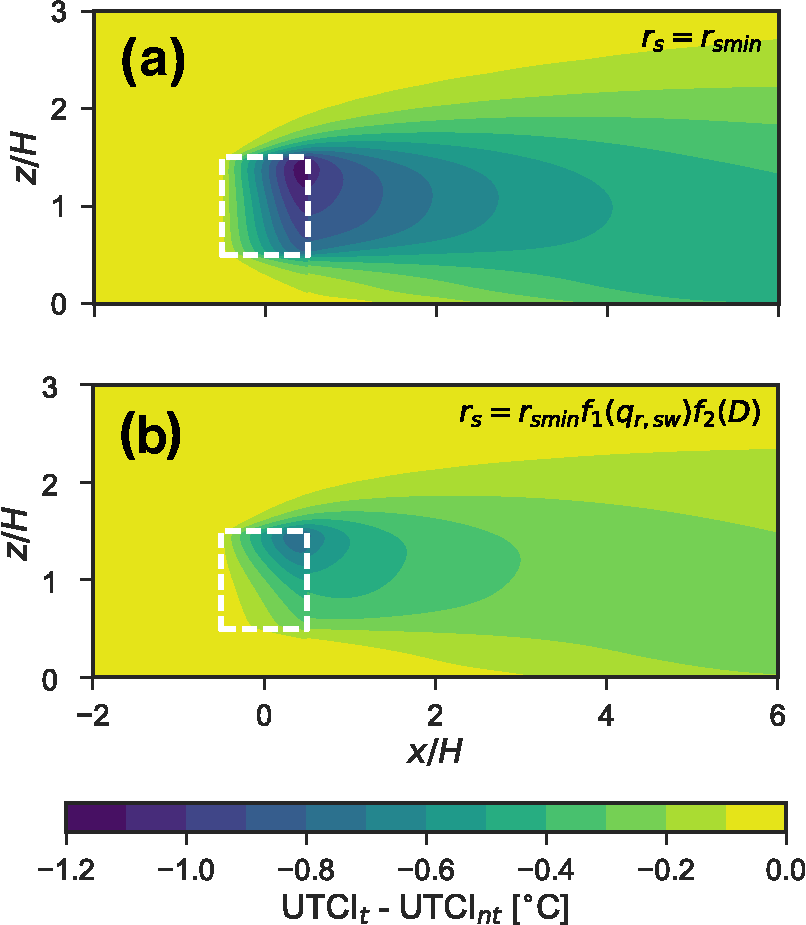
\includegraphics[height=0.6\textheight]{\figdir/utci_part2-crop.pdf}
		\caption{UTCI difference between transpiring and non-transpiring conditions, $\textit{UTCI}_t-\textit{UTCI}_{\textit{nt}}$  ($^{\circ}$C), for \subfig{a} constant stomatal resistance and \subfig{b} varying stomatal resistance.}
		\label{fig:utcifield2}
	\end{figure}

\cref{fig:utcifield1} shows the transpirative cooling effect of a tree row for fixed and varying stomatal resistance conditions. The figure compares transpiring (when stomata are open and transpiration from trees is enabled) and non-transpiring conditions (when stomata are closed and transpiration from trees is disabled). \cref{fig:utcifield1}a shows the UTCI ($^{\circ}$C) distribution during non-transpiring condition. As transpiration does not occur, the UTCI is the same for fixed and varying stomatal resistance. The figure shows that at the upstream region, where the flow is unaffected by the tree ($x/H=-2$ m), the UTCI reduces with height. The decrease of the UTCI with height is caused by the increase of wind speed with height. The figure also shows that the lowest value of the UTCI occurs inside and below the trees as it provides shading from the sun. The UTCI drops from $36$ $^{\circ}$C, a regime of strong heat stress, to $29$ $^{\circ}$C where the heat stress is moderate. Therefore, the trees have a large influence on the UTCI due to the shadowing effect from the solar radiation. This observation is in good agreement with field measurements of a rooftop garden in Singapore by \cite{Wong2003} where a large reduction in air temperature due to shading is also observed directly below the foliage. In the non-transpiring condition, we see that downstream of the trees, the UTCI increases, especially near the top region of the trees where most solar radiation is absorbed and the air temperature leaving the trees is higher. The absorbed radiation is balanced only with the sensible heat flux. The trees dissipate the energy simply through thermal exchanges leading to an increase in UTCI. Therefore, in an environmental condition such as drought, trees are unable to provide cooling through transpiration. Water availability is a key aspect for trees to form an effective cooling measure in urban areas. This can be challenging for cities as regular irrigation in summer, especially during heat waves, can further exacerbate the water demand and additionally, increase the cost of maintenance. 

\cref{fig:utcifield1}b and \cref{fig:utcifield1}c show the UTCI during the transpiring condition for fixed and varying stomatal resistances, respectively. We see that, for both cases, transpiration from the trees is beneficial as it reduces the UTCI compared to the non-transpiring condition. \cref{fig:utcifield2} shows the difference in UTCI between transpiring and non-transpiring conditions by calculating $\textit{UTCI}_t-\textit{UTCI}_{\textit{nt}}$ ($^{\circ}$C). Comparing the fixed and varying stomatal resistance cases, \cref{fig:utcifield2}a and \cref{fig:utcifield2}b respectively, we see that the varying stomatal case provides slightly less reduction in UTCI. Referring to the energy balance, and its results on \cref{fig:profiles}, the stomatal resistance is seen to increase towards the bottom of the foliage thereby reducing transpiration and increasing the leaf temperature. The region with the most transpirative cooling is the near-downstream region of the trees. This correlates with the observation of temperature and humidity distribution observed in \cref{fig:flowfields}. At higher stomatal resistance, the transpirative cooling is reduced due to the reduced latent heat flux. In the end, we see that the factor most contributing to improve pedestrian comfort is the shadowing provided by the trees, providing much lower UTCI than the transpirative cooling effect. 

\section{Influence of environmental factors}

A parametric study is performed on the influence of environmental conditions on the transpirative cooling effect of a single row of trees. The influence of environmental factors, i.e. wind speed $U_{\textit{ref}}$, air temperature $T$, relative humidity $\textit{RH}$ and solar radiation $q_{\textit{r,sw}}$ is studied by varying them independently \cref{tab:environmentalcond}. The impact of these environmental factors are determined by studying the energy exchanges at the leaf surface, the air temperature and the UTCI. The air temperature $T$ and the UTCI are evaluated at three distinct locations: \textit{upstream}, \textit{downstream} and in the \textit{shaded} region, as depicted in \cref{fig:domain}. The upstream region is unaffected by the trees, the downstream region is only affected by the transpiration and, finally, the shaded region shows the influence of shading from sun. 

\subsection{Influence of wind speed}

The wind speed has a direct influence on the convective transfer coefficients at the leaf surface. Due to this, wind speed also has an impact on the cooling effect of the trees. Therefore, the heat exchanges and the resulting cooling of the environment is studied for various wind speeds. The influence of wind speed on the net energy at the leaf is shown in \cref{fig:environmentalfactorspart1}a. A negative sensible heat flux indicates that heat is being extracted from the air and, therefore, cooling of the air occurs. The figure shows that the magnitude of the heat fluxes is increasing with wind speed. At high wind speed, the aerodynamic resistance \textbf{(Eq. (15))} reduces and leads to an increase in CHTC (\cref{eq:sensibleheatflux}) and CMTC (\cref{eq:latentheatflux}). We also observe that, at high wind speeds, the heat fluxes become less sensitive to wind speed. Therefore, it indicates that cooling by the trees becomes less sensitive to wind speed at higher wind speeds due to the power-law relation of CHTC and wind speed. 

	\begin{figure}[t]
	\centering
	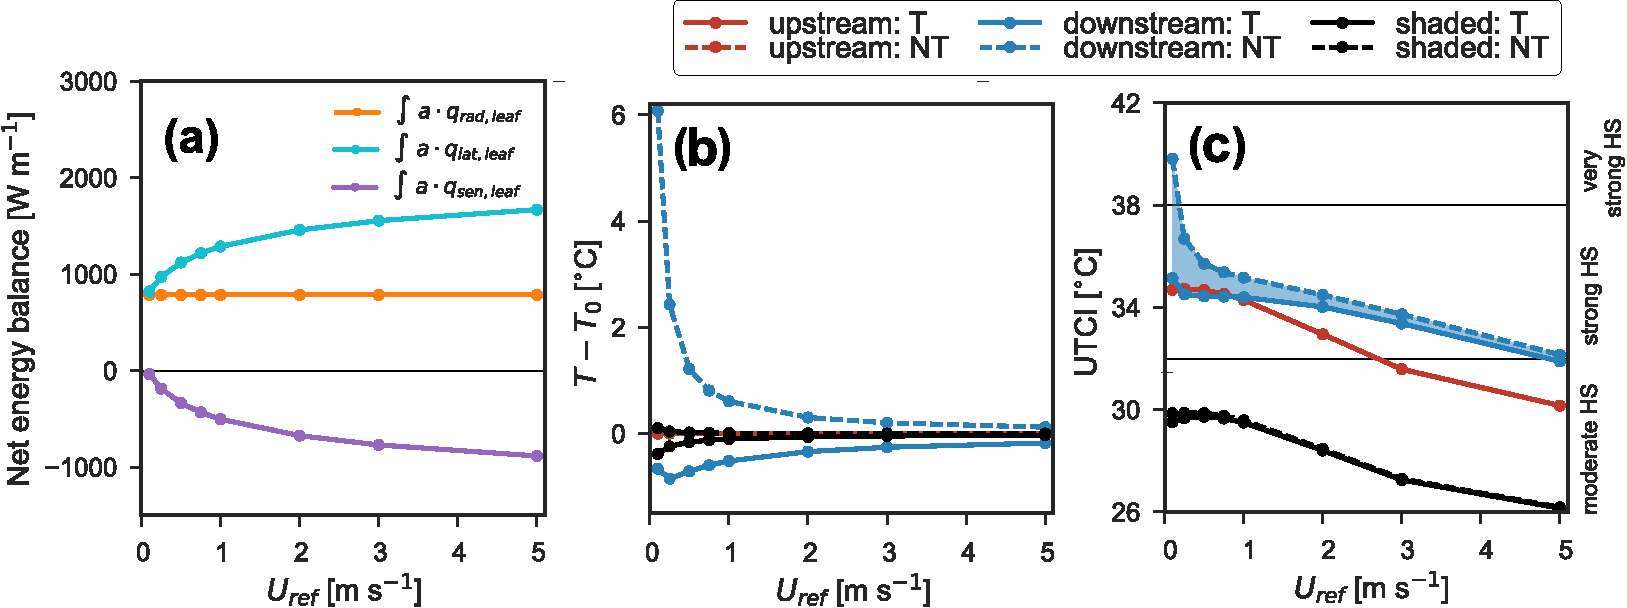
\includegraphics[width=\textwidth]{\figdir/environmentalfactors_type2_part1-crop.pdf}
	\caption{Influence of wind speed (m\,s$^{-1}$) on \subfig{a}  on the net energy balance of radiation, sensible and latent heat fluxes at the trees, $\int a \cdot (q_{\textit{rad,leaf}}-q_{\textit{sen,leaf}}-q_{\textit{lat,leaf}})\ dA = 0$ (W\,m$^{-1}$), \subfig{b} on air temperature $T-T_0$ ($^{\circ}$C), and \subfig{c} on $\textit{UTCI}$ ($^{\circ}$C). Point measurement of air temperature and $UTCI$ at three locations as shown in \cref{fig:domain}: \textit{upstream} ({\color{flatuidarkred}\textbf{red}}), \textit{downstream} ({\color{flatuidarkblue}\textbf{blue}}) and \textit{shaded} (\textbf{black}) for transpiring (T) (solid, ---) and non-transpiring (NT) conditions (dashed, - - -).}
	\label{fig:environmentalfactorspart1}
	\end{figure}
	
\cref{fig:environmentalfactorspart1}b shows the air temperature difference between the inlet and three distinct locations $(T-T_0)$: \textit{upstream}, \textit{downstream} and \textit{shaded}, as depicted in \cref{fig:domain}. In addition, the air temperature is compared for the transpiring (T) and non-transpiring (NT) conditions, to indicate the influence of transpirative cooling. The upstream region is unaffected by the trees and remains constant for transpiring and non-transpiring conditions. In the shaded region, the transpirative cooling has only a small influence as there is no cold air transported downwards from the trees. For the non-transpiring condition, the air temperature increases slightly at lower wind speeds. For the transpiring condition, the air temperature reduces by $0.4$ $^{\circ}$C. In the downstream region, the influence of the trees on the air temperature is clearly visible, with a large increase in air temperature for the non-transpiring condition, up to 6 $^{\circ}$C, and significant drop in air temperature for the transpiring condition, approximately $-0.9$ $^{\circ}$C at the wind speed of $0.25$ m\,s$^{-1}$. \cref{fig:environmentalfactorspart1}b also shows that air cooling downstream of the trees decreases with increasing wind speed. \cite{Dimoudi2003} also provide similar finding in their CFD study of vegetation in urban environment, where the effect of vegetation seems to decrease with increasing wind speed. This occurs as, for higher wind speeds, the trees extract a similar amount of heat per second from a larger air volume, resulting in a smaller overall temperature reduction. At low wind speeds, the heat extraction is done over a small volume or air, i.e., a lower flow rate, providing a larger temperature reduction. Similarly, during non-transpiring conditions, the air temperature substantially increases near the trees, since in this case the radiative heat is not converted into latent heat, but convected as sensible heat into the air domain. Therefore, when the goal is to provide maximum reduction in air temperature in the vicinity of the tree row, lower wind speeds are preferable. As such, at low wind speeds, a local cool region is created around the vegetation. However, at higher wind speeds, the total amount of sensible heat that is extracted from the flow by transpiration is larger. Thus, for global heat island mitigation, high wind speeds are more beneficial, while low wind speeds are favorable to improve the local thermal comfort around a tree.

\cref{fig:environmentalfactorspart1}c shows the UTCI in transpiring and non-transpiring conditions. For both conditions, the UTCI reduces with increasing wind speed at all locations, as expected. The upstream probe point shows that high wind speeds result in a reduced UTCI as wind speed has a direct influence on the comfort. The heat stress levels reduce from strong heat stress (HS) to moderate HS. This characteristic is also visible for the downstream and the shaded probe point. However, the shaded probe point is always in moderate HS levels for all wind speeds. This is due to the reduced radiation levels, indicating the importance of shading provided by the trees yielding a $4-6$ $^{\circ}$C reduction in the UTCI. The impact of transpirative cooling is visible by studying the difference between transpiring and non-transpiring conditions, $\textit{UTCI}_t-\textit{UTCI}_{\textit{nt}}$ (indicated in shaded area). The figure shows that the transpirative cooling provided by the trees, i.e. $\textit{UTCI}_t-\textit{UTCI}_{\textit{nt}}$, only has an impact downstream of the tree row as it is negligible at both upstream and shaded regions. At low wind speeds, the transpirative cooling is the largest whereas, at higher wind speeds, the impact of transpirative cooling on the UTCI is negligible. This indicates that a pedestrian downstream of a tree row only notices the benefit of transpirative cooling when wind speeds are low. However, vegetation extracts more heat from the environment when wind speeds are higher.

\subsection{Influence of relative humidity and air temperature}

				
	\begin{figure}[t]
		\centering
		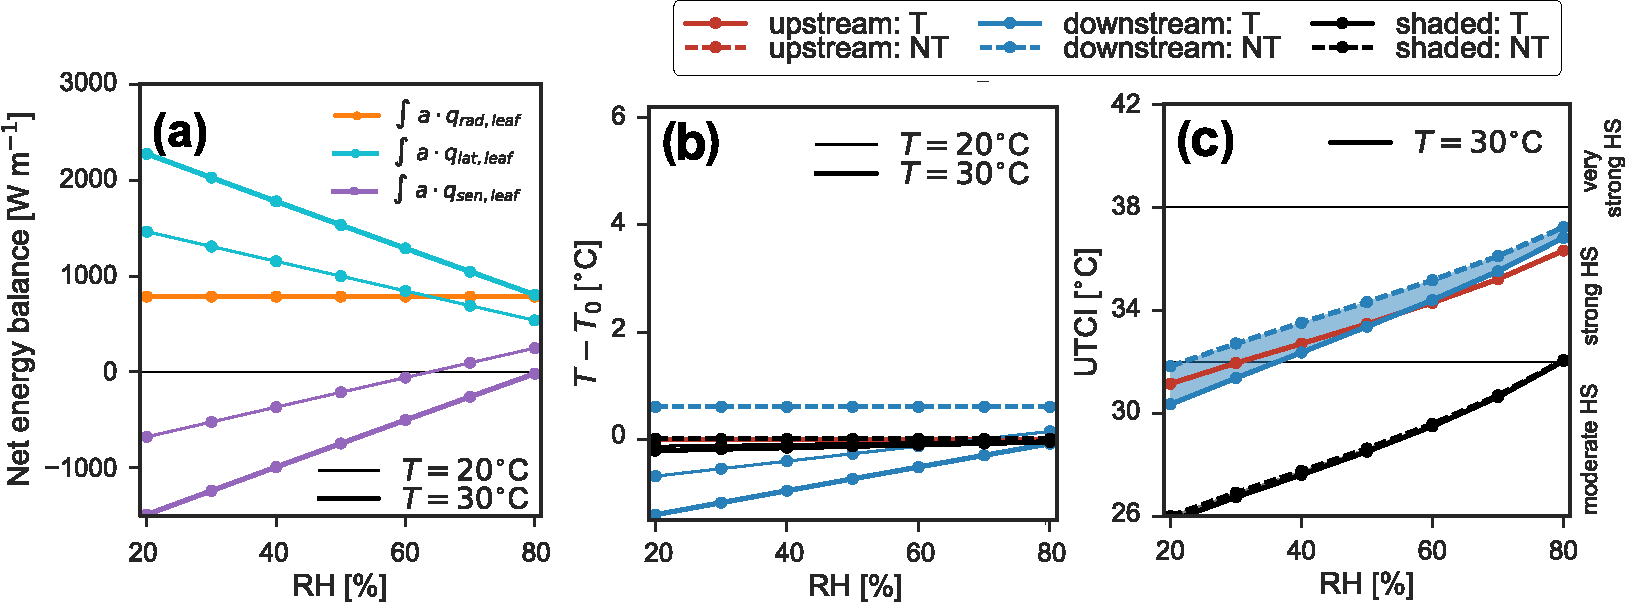
\includegraphics[width=\textwidth]{\figdir/environmentalfactors_type2_part2-crop.pdf}
		\caption{Influence of relative humidity $RH$ (\%) at air temperature $T=20$ $^{\circ}$C (thin) and $T=30$ $^{\circ}$C (thick) on \subfig{a} on the net energy balance of radiation, sensible and latent heat fluxes at the trees, $\int a \cdot (q_{\textit{rad,leaf}}-q_{\textit{sen,leaf}}-q_{\textit{lat,leaf}})\ dA = 0$ (W\,m$^{-1}$), \subfig{b} on air temperature $T-T_0$ ($^{\circ}$C), and \subfig{c} on $\textit{UTCI}$ ($^{\circ}$C). Point measurement of air temperature and $UTCI$ at three locations as shown in \cref{fig:domain}: \textit{upstream} ({\color{flatuidarkred}\textbf{red}}), \textit{downstream} ({\color{flatuidarkblue}\textbf{blue}}) and \textit{shaded} (\textbf{black}) for transpiring (T) (solid, ---) and non-transpiring (NT) conditions (dashed, - - -).}
		\label{fig:environmentalfactorspart2}
	\end{figure}

The vapor pressure varies depending on relative humidity ($RH$) and air temperature $T$. A variation in vapor pressure of the air has a direct influence on the rate of transpiration, since mass flux from leaf surface is driven by the gradient in vapor pressure between the leaf surface and the ambient air. As a result, RH and ambient air temperature have a direct influence on the cooling power of the tree row. \cref{fig:environmentalfactorspart2}a shows the influence of RH and air temperature on the heat exchanges. We observe that, at low RH, the magnitudes of the latent and sensible heat fluxes are high. This indicates high transpiration rate and similarly large cooling, as indicated by the downstream probe point in transpiring conditions, as seen in \cref{fig:environmentalfactorspart2}b. However, at high RH, the transpiration is much lower and results in a higher leaf temperature leading to heating of the air. This is due to air vapor pressure approaching saturation resulting in a reduced capacity for air to take up additional humidity from the leaves. At lower air temperature, $T=20$ $^{\circ}$C, the saturation vapor pressure of the air is lower and, therefore, the air has less capacity to take in the humidity from the leaves. With a reduced transpiration rate, the latent heat flux is reduced, leading to higher air temperature (\cref{fig:environmentalfactorspart2}b). Thus, we see that the trees provide the maximum cooling during hot dry conditions providing approximately 4.5 times larger air temperature drop (at $T=30$ $^{\circ}$C and $\textit{RH}=20$ \%) than the colder humid condition (at $T=20$ $^{\circ}$C and $RH=80$ \%).

\cref{fig:environmentalfactorspart2}c shows the influence of RH on thermal comfort at $T=30$ $^{\circ}$C. With increasing RH from dry to humid conditions, the UTCI increases from a moderate to a strong heat stress regime. This effect is independent of the trees as RH and temperature play themselves also a direct role on the thermal comfort as high humidity results in lower comfort for a pedestrian. Studying the influence of transpirative cooling, we see that the shaded and upstream locations are unaffected, showing a negligible $\textit{UTCI}_t-\textit{UTCI}_{\textit{nt}}$. However, we note that transpirative cooling consistently improves thermal comfort in the downstream region, with a greater influence in the dry condition. At higher RH, even though transpiration reduces the UTCI, the UTCI downstream of the tree row is higher than the upstream region. However, this does not indicate that the presence of trees is detrimental, as the thermal influence of the ground is not modeled in the present study. The trees provide shading to the ground and we recall that the resulting additional cooling due to lower ground temperature is not taken into account in the present study. 

\subsection{Influence of solar radiation intensity}

The net absorbed solar radiation, $\int a q_{\textit{rad,leaf}}\ dV$, has a direct influence on the transpiration rate from the leaves. \cref{fig:environmentalfactorspart3}a shows the influence of solar radiation on the energy balance. The magnitude of the latent heat flux increases with increasing solar radiation. However, we notice that, even though there is a higher transpiration rate from the trees (as CMTC is constant), the sensible heat flux becomes more positive resulting in less cooling, as depicted in \cref{fig:environmentalfactorspart3}b. This indicates that, at high solar radiation, the transpiration rate is not sufficiently high to ensure cooler leaves as seen in the low radiation intensity case. Studying the temperature variations in the upstream and the shaded regions, no influence of radiation on transpirative cooling is seen. 
	
\begin{figure}[t]
	\centering
	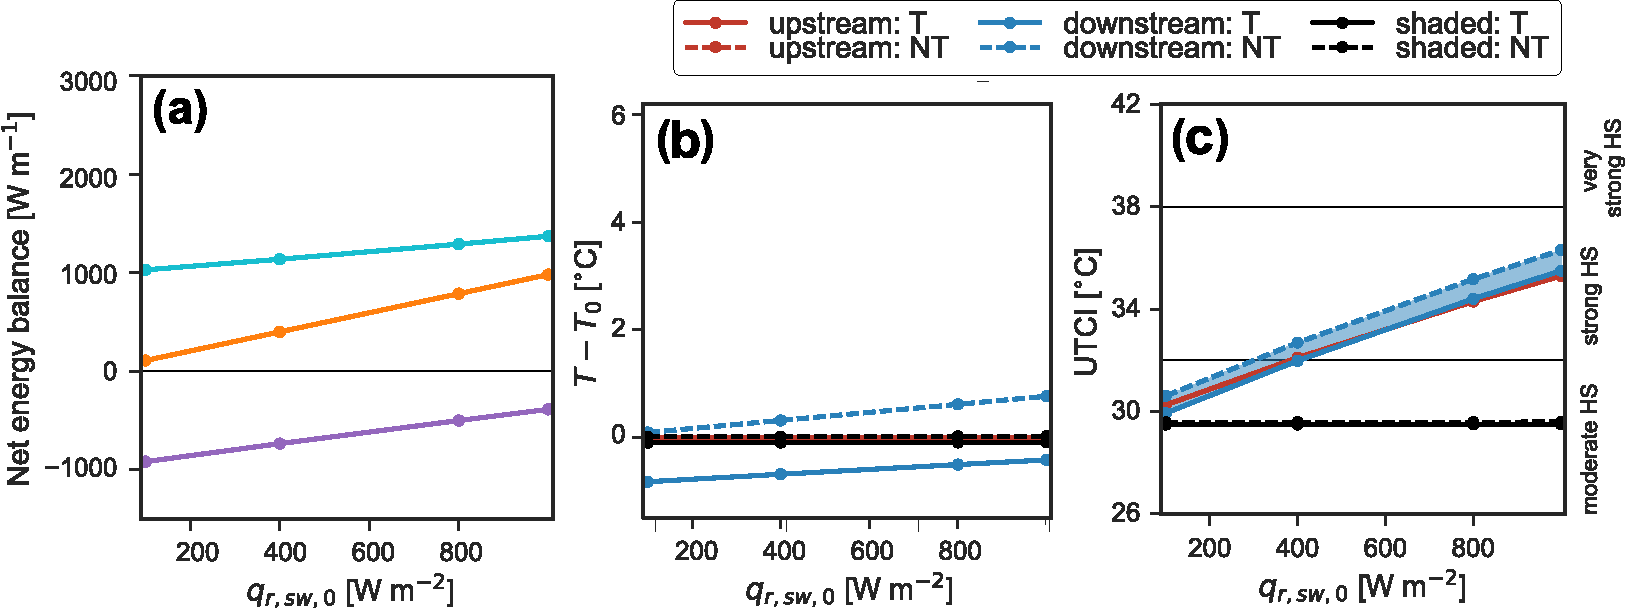
\includegraphics[width=\textwidth]{\figdir/environmentalfactors_type2_part3-crop.pdf}
	\caption{Influence of solar radiation $q_{\textit{r,sw,0}}$ (W\,m$^{-2}$) on \subfig{a} on the net energy balance of radiation, sensible and latent heat fluxes at the trees, $\int a \cdot (q_{\textit{rad,leaf}}-q_{\textit{sen,leaf}}-q_{\textit{lat,leaf}})\ dA = 0$ (W\,m$^{-1}$), \subfig{b} on air temperature $T-T_0$ ($^{\circ}$C), and \subfig{c} on $\textit{UTCI}$ ($^{\circ}$C). The shaded region shows the difference $\textit{UTCI}_t-\textit{UTCI}_{\textit{nt}}$ ($^{\circ}$C). Point measurement of air temperature and $UTCI$ at three locations as shown in \cref{fig:domain}: \textit{upstream} ({\color{flatuidarkred}\textbf{red}}), \textit{downstream} ({\color{flatuidarkblue}\textbf{blue}}) and \textit{shaded} (\textbf{black}) for transpiring (T) (solid, ---) and non-transpiring (NT) conditions (dashed, - - -).}
	\label{fig:environmentalfactorspart3}
\end{figure}

\cref{fig:environmentalfactorspart3}c shows the influence of solar radiation on thermal comfort. The UTCI in both the downstream region and the upstream regions is almost similar. At both locations, the UTCI increases from moderate HS to strong HS simply due to the higher value of solar radiation. The transpirative cooling effect, indicated by $\textit{UTCI}_t-\textit{UTCI}_{\textit{nt}}$, is nearly constant at all solar radiation levels. Therefore, we see that the transpirative cooling provided by the trees is weakly dependent on the solar radiation. In the shaded region indicated by the black line, the UTCI is much lower and is independent of the solar radiation due to the shadowing effect. 

\subsection{Summary on the impact of environmental factors}

For this case study, the transpirative cooling effect of a single row of trees is highest at lower wind speed when $U < 1$ m\,s$^{-1}$. At higher wind speed, the impact of wind speed on latent and sensible heat fluxes becomes weak and a non-linear dependency is only observed for wind speed (\cref{fig:environmentalfactorspart1}a). This also results in very small changing air temperature at higher wind speeds (\cref{fig:environmentalfactorspart1}b). Relative humidity and solar radiation result in a rather linear change in air temperature. We observe that a pedestrian locally notices the benefit of transpirative cooling when wind speeds are low as indicated by UTCI. However, the trees extract the maximum heat from the environment at high wind speeds. Thus, policies focused on mitigation of the citywide heat island effect should ensure that only trees with low blockage effect are planted and in well-ventilated areas. Whereas, policies aimed at creating oasis of cool areas should focus on making dense vegetation areas such as parks that can substantially reduce the wind speed. Furthermore, we also observe that the trees provide the largest cooling effects during hot conditions with low RH. However, to ensure this transpirative cooling, the plants need to be well irrigated, which can be difficult in hot and dry cities. Therefore, in such climatic conditions, cities can focus on developing parks and similar dense localized vegetated areas that not only create oases of cool and humid areas but also the irrigation of such areas can be more efficient. Whereas, in humid conditions, the transpirative cooling effect is negligible and the comfort is only improved by the shadowing effect. Therefore, cities with hot and humid conditions should focus on integrating tall-wide canopy trees that can maximize the shadowing effect. 

\section{Influence of tree properties}

The influence of tree properties on the transpirative cooling effect of a tree row is investigated by varying the leaf size $l$, minimum stomatal resistance $r_{\textit{s,min}}$ and the leaf area density $a$. 

\subsection{Influence of leaf size}

\cref{fig:treefactorspart1}a shows the impact of leaf size on the energy balance. The figure shows that the sensible and latent fluxes reduces in strength with increasing leaf size. The behavior is due to inverse relation of CHTC (\cref{eq:sensibleheatflux}) and CMTC (\cref{eq:latentheatflux}) with leaf size. A large leaf size results in reduced heat and mass fluxes from the trees, yielding the reduced cooling seen in \cref{fig:treefactorspart1}b. The highest cooling effect is observed when leaf size is small since CHTC and CMTC are then higher, when convective transfer is more efficient. This is also evident from field measurements of forest trees where smaller-leaves species is observed to be cooler\citep{Leuzinger2007,Leuzinger2010}. The influence of transpirative cooling is negligible in the upstream and shaded region and the thermal comfort, indicated by UTCI is nearly unaffected by the leaf size, \cref{fig:treefactorspart1}c. Even though there is a variation in the air temperature (\cref{fig:treefactorspart1}b), the UTCI is relatively unaffected as there is also an increase in humidity downstream of the trees, countering the benefit provided by the reduced air temperature. The use of leaf size in determining CHTC and CMTC shows that a higher developing length, resulting in a larger aerodynamic resistance over the leaf surface, reduces convective exchanges.


	\begin{figure}[t]
	\centering
	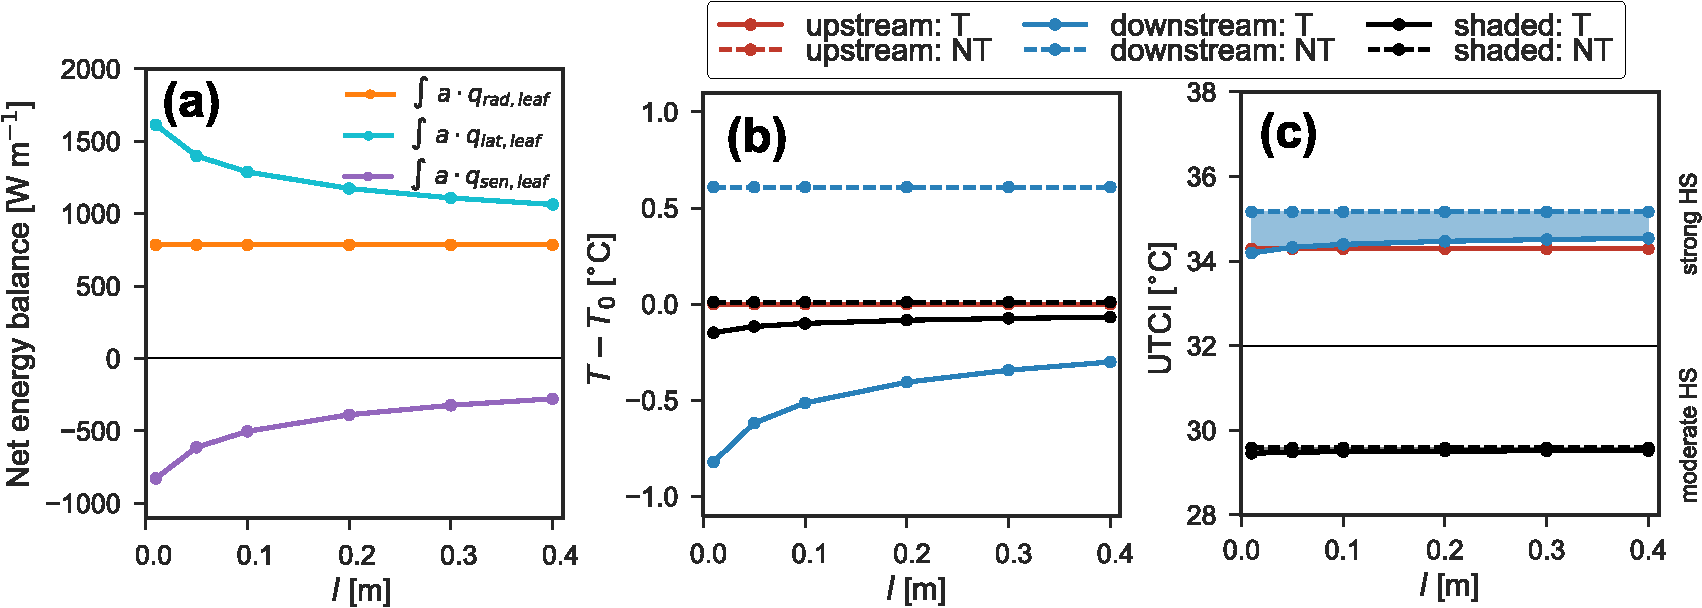
\includegraphics[width=\textwidth]{\figdir/treefactors_type2_part1-crop.pdf}
	\caption{Influence of leaf size $l$ (m) \subfig{a} on the net energy balance of radiation, sensible and latent heat fluxes at the trees, $\int a \cdot (q_{\textit{rad,leaf}}-q_{\textit{sen,leaf}}-q_{\textit{lat,leaf}})\ dA = 0$ W\,m$^{-1}$, \subfig{b} on air temperature $T-T_0$ ($^{\circ}$C), and \subfig{c} $\textit{UTCI}$ ($^{\circ}$C). Point measurement of air temperature and $UTCI$ at three locations as shown in \cref{fig:domain}: \textit{upstream} ({\color{flatuidarkred}\textbf{red}}), \textit{downstream} ({\color{flatuidarkblue}\textbf{blue}}) and \textit{shaded} (\textbf{black}) for transpiring (T) (solid, ---) and non-transpiring (NT) conditions (dashed, - - -).}
	\label{fig:treefactorspart1}
	\end{figure}

\subsection{Influence of stomatal resistance}

The stomatal resistance has a larger influence on the heat and mass fluxes than the leaf sizes as shown in \cref{fig:treefactorspart2}a. As CMTC is inversely dependent on the stomatal resistance, increasing the stomatal resistance causes the transpiration from the leaf to decrease. Less transpiration leads to less heat removal causing an increase of leaf temperature and a reduced cooling effect, as shown in \cref{fig:treefactorspart2}b. Therefore, plants with low stomatal resistance such as the impatiens plant or grass can provide more cooling than deciduous plant, for similar leaf sizes and leaf area densities. \cref{fig:treefactorspart2}c shows that stomatal resistance has a weak influence on the UTCI. As seen with leaf size, a stomatal resistance variation results in a negligible change in UTCI downstream of the trees as the lower air temperature is counter-balanced with higher air humidity. However comparing the transpiring and non-transpiring cases, we see that transpiration still provides an improvement in thermal comfort showing a positive difference $\textit{UTCI}_t-\textit{UTCI}_{\textit{nt}}$, \cref{fig:treefactorspart2}c.

	\begin{figure}[t]
		\centering
		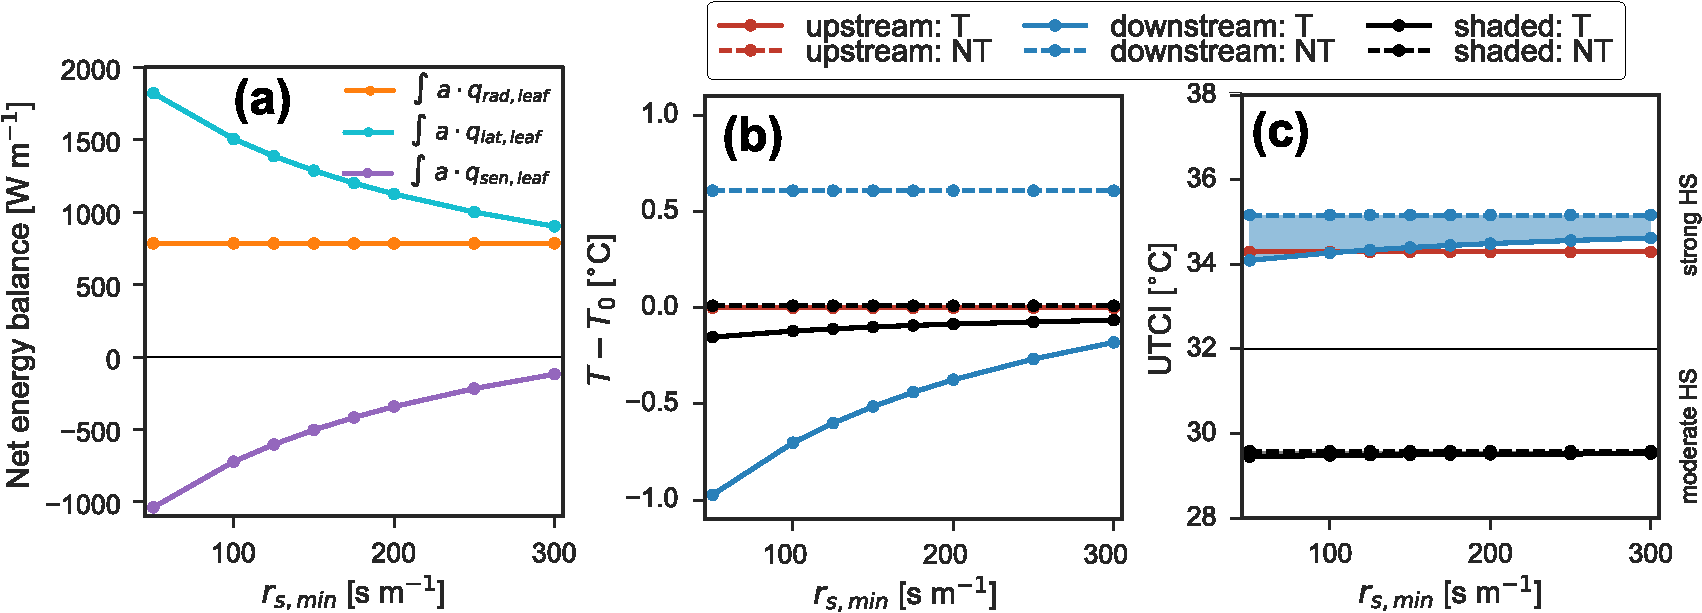
\includegraphics[width=\textwidth]{\figdir/treefactors_type2_part2-crop.pdf}
		\caption{Influence of stomatal resistance $r_{\textit{s,min}}$ (s\,m$^{-1}$) on \subfig{a} the net energy balance of radiation, sensible and latent heat fluxes at the trees, $\int a \cdot (q_{\textit{rad,leaf}}-q_{\textit{sen,leaf}}-q_{\textit{lat,leaf}})\ dA = 0$ W\,m$^{-1}$, \subfig{b} on air temperature $T-T_0$ ($^{\circ}$C), and \subfig{c} $\textit{UTCI}$ ($^{\circ}$C). Point measurement of air temperature and $UTCI$ at three locations as shown in \cref{fig:domain}: \textit{upstream} ({\color{flatuidarkred}\textbf{red}}), \textit{downstream} ({\color{flatuidarkblue}\textbf{blue}}) and \textit{shaded} (\textbf{black}) for transpiring (T) (solid, ---) and non-transpiring (NT) conditions (dashed, - - -).}
		\label{fig:treefactorspart2}
	\end{figure}

\subsection{Influence of leaf area density}

\cref{fig:treefactorspart3}a shows that, when leaf area density is low, the net radiation absorbed by vegetation is lower due to the lack of leaf surfaces to absorb the radiation, which means more solar radiation can passes through the vegetation. \cref{fig:treefactorspart3}b shows that there is a decrease in the UTCI in the shaded region with higher leaf density, which increases shading of solar radiation. In the case of low leaf area density, more leaf surfaces are exposed to a higher solar radiation over the whole volume of vegetation, resulting in higher air temperature while the transpiration rate is not sufficient to cool the leaves, \cref{fig:treefactorspart3}c. \cite{Hiraoka2005} also observes that, for a single tree with leaf area density $a=1$, at environmental condition of $T=30$ $^{\circ}$C and $\textit{RH}=80$ \%, sensible heat is added to the air domain. However, with a higher leaf area density, more solar radiation is absorbed at the top of the vegetation, shading the lower regions from the solar radiation. This is beneficial as leaf surfaces at lower regions are then able to dissipate the absorbed solar radiation through transpiration and to cool the air. Therefore, the leaf area density should be sufficiently high such that solar radiation is mostly absorbed at the top of the vegetation volume. 

	\begin{figure}[t]
	\centering
	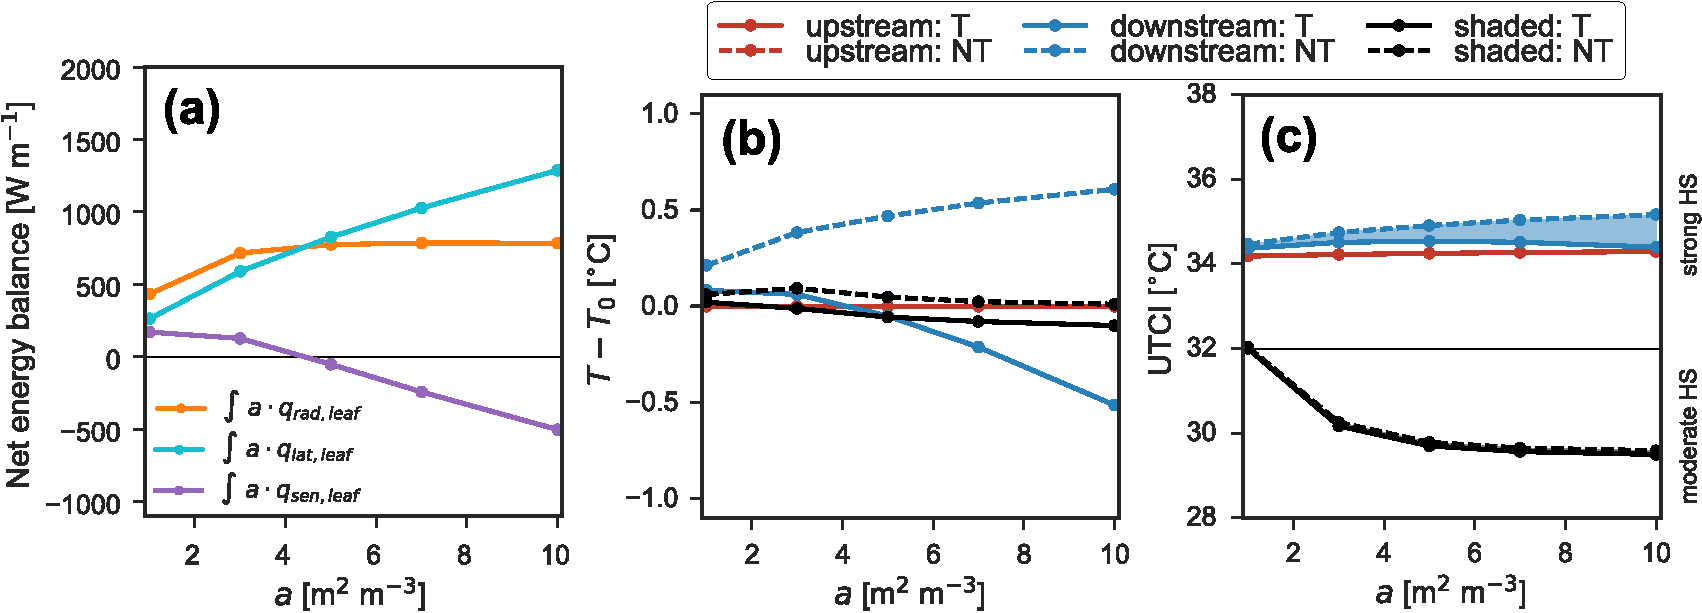
\includegraphics[width=\textwidth]{\figdir/treefactors_type2_part3-crop.pdf}
	\caption{Influence of leaf area density $a$ (m$^{2}$\,m$^{-3}$) on \subfig{a} the net energy balance of radiation, sensible and latent heat fluxes at the trees, $\int a \cdot (q_{\textit{rad,leaf}}-q_{\textit{sen,leaf}}-q_{\textit{lat,leaf}})\ dA = 0$ W\,m$^{-1}$, \subfig{b} on air temperature $T-T_0$ ($^{\circ}$C), and \subfig{c} $\textit{UTCI}$ ($^{\circ}$C). Point measurement of air temperature and $UTCI$ at three locations as shown in \cref{fig:domain}: \textit{upstream} ({\color{flatuidarkred}\textbf{red}}), \textit{downstream} ({\color{flatuidarkblue}\textbf{blue}}) and \textit{shaded} (\textbf{black}) for transpiring (T) (solid, ---) and non-transpiring (NT) conditions (dashed, - - -).}
	\label{fig:treefactorspart3}
	\end{figure}

\subsection{Summary on the influence of tree properties}

The study on the influence of tree properties on the net energy balance shows that both leaf size and stomatal resistance have a non-linear effect. Both leaf size and stomatal resistance influence the convective heat and mass transfer coefficients at the surface of leaves. Plants with larger leaves provide less cooling effect than plant with small leaves, \cref{fig:treefactorspart2}a. We also observe that, to provide the highest cooling, the stomatal resistance should be low such that transpiration rate is high. However, higher rate of transpiration results also in increased humidity in the air and counters the thermal comfort provided by reduced air temperature. The study on the impact of leaf area density shows that leaf area density should be sufficiently high such that solar radiation is mostly absorbed at the top of the vegetation volume. Therefore, the lower part of the volume are shaded and can provide cooling to the air. A similar observation is found in the field measurements of rooftop gardens in Singapore where thicker foliated plants are shown to provide more cooling \citep{Wong2003}. The cooling provided by the single row of trees is seen to grow almost linearly with leaf area density providing 10 times higher temperature drop and UTCI drop for a densely foliated tree row of $a=10$ m$^2$~m$^{-3}$ compared to a weakly foliated tree row of $a=1$ m$^2$~m$^{-3}$. Therefore, cities focused on mitigating UHI through shading of vegetation should ensure that the trees are sufficiently foliated to reduce the transmission of short-wave radiation through vegetation. 

\section{Influence of vegetation size}

Finally we investigate how vegetation size influences the transpirative cooling effect. The size of vegetation in the domain can be described in terms of its length, i.e. number of tree rows $n$, or the height of the trees $n\,H$ as shown in \cref{fig:domainvegsize}. The impact of the tree height on the air temperature is determined by probing the \textit{upstream} region $\left(x = -H,\, y = H\right)$, the \textit{shaded} region $\left(x = 0,\, y = H/4\right)$ and the \textit{downstream} region $\left(x=H,\, y=H \right)$ at fixed heights. The probe locations have fixed heights as they represent a reference pedestrian standing next to trees with varying heights. The impact of number of tree rows on the air temperature is determined for three positions: \textit{upstream} $\left(x=-H,\, y=H \right)$, \textit{shaded} $\left(x=0,\, y=H/4 \right)$ and downstream region $\left( x= nH+H,\, y=H\right)$. The downstream probe point is located at distance $H$ away from the last downwind tree row.

	\begin{figure}[p]
		\centering
		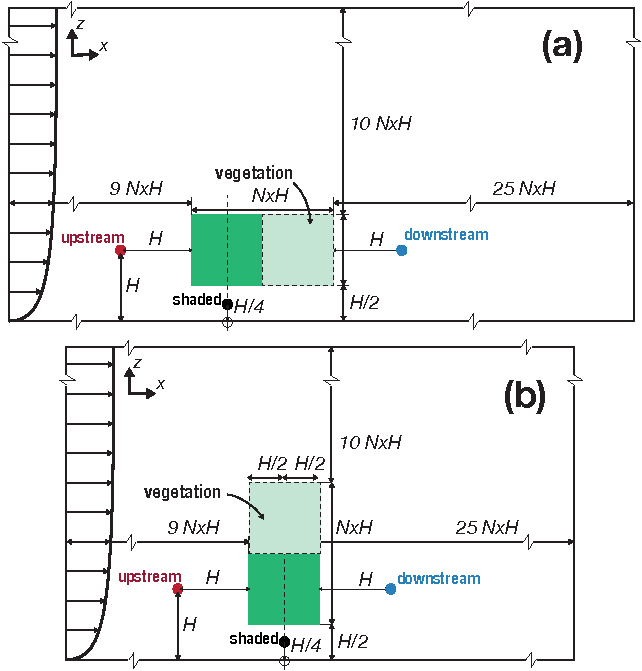
\includegraphics[width=\textwidth]{\figdir/domain_treeHeight-crop.pdf}
		\caption{Simulation domain for the study on the size of vegetation, where vegetation region is indicated in green ({\color{flatuidarkgreen}$\blacksquare$}), \subfig{a} study on the number of tree rows $n=[1,2,5,10]$, and \subfig{b} study on the tree height $n\,H$ with $n=[1,2,3,5,10]$. The sample points at three locations: \textit{upstream} ({\color{flatuidarkred}\textbf{red}}), \textit{downstream} ({\color{flatuidarkblue}\textbf{blue}}) and \textit{shaded} (\textbf{black}).}
		\label{fig:domainvegsize}
	\end{figure}

\subsection{Influence of number of tree rows}

A study on the influence of the number of tree rows provides an understanding on how increasing vegetation along the downstream direction has an effect on the overall cooling of the environment. \cref{fig:vegetationsizepart1}a shows the influence of number of tree rows on the net energy balance. The net absorbed radiation is linearly increasing with number of tree rows. The latent heat flux increases as well whereas the sensible heat flux approaches zero. Despite an increase in net transpiration, the cooling reduces. Since each additional tree row results in a lower wind speed due to the increased momentum drag, the lower CHTC and CMTC result in a reduction of transpiration and a reduced cooling of the air downstream of the tree row \cref{fig:vegetationsizepart1}b. When the trees does not transpire, an increase in the number of tree rows causes more heating of the flow. Reversely, transpiration ensures that the air domain is cooled regardless of the number of tree rows. The study of the impact of number of tree rows on the thermal comfort \cref{fig:vegetationsizepart1}c shows that there is large change in the thermal comfort comparing transpiring and non-transpiring conditions. The transpirative cooling provided by the trees regulates the thermal comfort downstream of the tree row. The absence of transpiration yields growing deterioration of the thermal comfort with an increasing number of tree rows. Thus, the transpirative cooling effect plays a critical role when increasing the number of tree rows in the domain. 

	\begin{figure}[t]
	\centering
	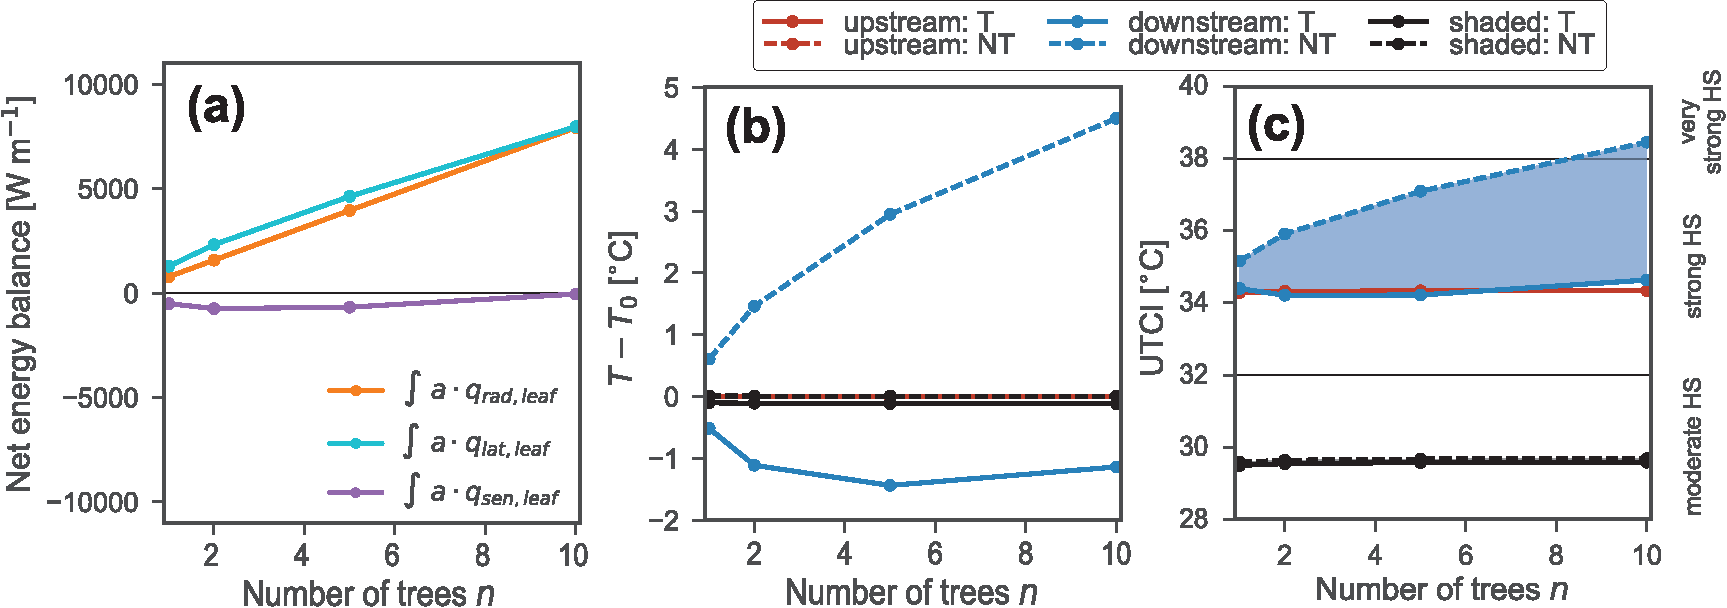
\includegraphics[width=\textwidth]{\figdir/vegetationsize_type2_part1-crop.pdf}
	\caption{Influence of number of tree rows $n$ on \subfig{a} the net energy balance of radiation, sensible and latent heat fluxes at the trees, $\int a \cdot (q_{\textit{rad,leaf}}-q_{\textit{sen,leaf}}-q_{\textit{lat,leaf}})\ dA = 0$ W~m$^{-1}$, \subfig{b} on air temperature $T-T_0$ ($^{\circ}$C), and \subfig{c} $\textit{UTCI}$ ($^{\circ}$C). Point measurement of air temperature and $UTCI$ at three locations as shown in \cref{fig:domainvegsize}: \textit{upstream} ({\color{flatuidarkred}\textbf{red}}), \textit{downstream} ({\color{flatuidarkblue}\textbf{blue}}) and \textit{shaded} (\textbf{black}) for transpiring (T) (solid, ---) and non-transpiring (NT) conditions (dashed, - - -).}
	\label{fig:vegetationsizepart1}
	\end{figure}

\subsection{Influence of tree height}

\cref{fig:vegetationsizepart2}a shows the influence of tree height on the net energy balance. The solar radiation absorbed by the trees does not change with increasing height as the top of the trees has absorbed all the incident solar radiation independently from tree height. However, the magnitudes of latent and sensible heat fluxes increase linearly with tree height as there is a linear increase of leaf surfaces, thus in transpirative cooling effect. \cref{fig:vegetationsizepart2}b shows that the cooling of the air at the downstream location converges to $-1$ $^{\circ}$C in the transpiring condition and, for the non-transpiring condition, the temperature change approaches zero. This occurs because the top of the trees, which is hotter, is further away from the pedestrian level. Therefore, at the lower regions of the trees, the magnitude of the sensible heat flux remains uniform in height, providing equal change in air temperature. This is also evident from observing the thermal comfort, \cref{fig:vegetationsizepart2}c.  The UTCI does not vary after the trees are higher than $3$ m. The shaded region can be assumed to be unaffected by the change in tree height as indicated by a negligible temperature change, \cref{fig:vegetationsizepart2}b, and a negligible UTCI change, \cref{fig:vegetationsizepart2}c.  

	\begin{figure}[t]
	\centering
	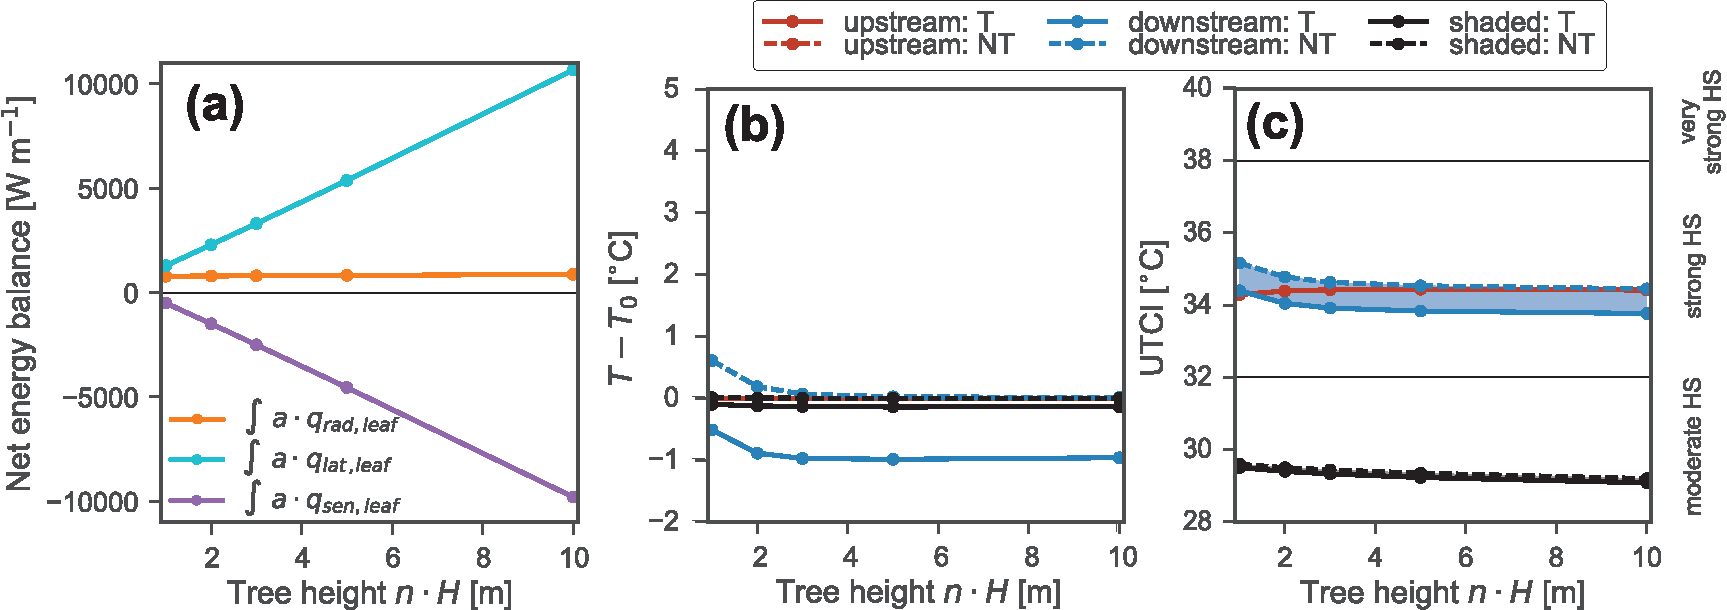
\includegraphics[width=\textwidth]{\figdir/vegetationsize_type2_part2-crop.pdf}
	\caption{Influence of tree height $n\,H$ (m) on \subfig{a} the net energy balance of radiation, sensible and latent heat fluxes at the trees, $\int a \cdot (q_{\textit{rad,leaf}}-q_{\textit{sen,leaf}}-q_{\textit{lat,leaf}})\ dA = 0$ W\,m$^{-1}$, \subfig{b} on air temperature $T-T_0$ ($^{\circ}$C), and \subfig{c} $\textit{UTCI}$ ($^{\circ}$C). Point measurement of air temperature and $UTCI$ at three locations as shown in \cref{fig:domainvegsize}: \textit{upstream} ({\color{flatuidarkred}\textbf{red}}), \textit{downstream} ({\color{flatuidarkblue}\textbf{blue}}) and \textit{shaded} (\textbf{black}) for transpiring (T) (solid, ---) and non-transpiring (NT) conditions (dashed, - - -).}
	\label{fig:vegetationsizepart2}
	\end{figure}

\subsection{Summary on the influence of vegetation size}

The study on the influence of vegetation size is performed by varying the tree height and the number of tree rows. An increase in the number of tree rows has an influence on the CHTC and the CMTC due to the reduction in wind speed. A reduced wind speed results in a lower transpiration leading to a reduced transpirative cooling effect of the air. We also observe that, when increasing the number of tree rows, if the trees does not transpire, the thermal comfort continues to deteriorate. Therefore, transpiration plays a critical role when increasing the number of tree rows. A study on the influence of tree height shows that the top of the trees, which is hotter and is far high enough from the ground, the thermal comfort at pedestrian level is higher. This indicates that ideally, cities should focus on implementing a combination of tall wide-canopy trees and dense foliated pedestrian-level trees. The tall wide-canopy trees can provide shading to the building surfaces, and the warmer leaves are also further away from the pedestrian level to not have a negative influence on the thermal comfort. Furthermore, the densely foliated pedestrian-level trees can provide transpirative cooling and generate cool oasis at the ground level.


\section{Conclusion}

In this study, we investigated the influence of environmental factors, tree properties and size on the transpirative cooling effect of a single row of trees. A computational fluid dynamics (CFD) model is used for modelling the flow in the air domain and through the vegetation. Vegetation is modelled as a porous medium where the heat exchange is solved using a leaf energy balance model. The long-wave radiative transfer between vegetation and the environment is empirically modelled. The vegetation model is validated against the numerical and experiment study of \cite{Kichah2012}. Thereafter, a parametric study is performed to determine the transpirative cooling effect of vegetation at noon with a solar altitude of $90^{\circ}$. The following conclusions were determined from the parametric study:

\begin{enumerate}
\item The transpirative cooling effect of a single row of trees is highest at lower wind speed when $U<1$ m\,s$^{-1}$. 
\item A pedestrian perceives transpirative cooling mainly when wind speeds are low, as indicated by the UTCI showing a cool zone locally around the trees. However, trees extract more sensible heat from the flow by transpiration when wind speeds are higher.
\item The transpirative cooling effect of a row of trees is diminished in humid and low temperature conditions, where the vapor pressure of air is closer to saturation and the transpiration from vegetation diminishes. Cities in such climatic condition should develop mitigation strategies focusing on cooling by shading and less on maximizing transpirative cooling.
\item Solar radiation has a large influence on the thermal comfort and, in all cases, the comfort level below the trees is substantially higher than downstream of the tree row due to shadowing effects. The additional benefit of transpirative cooling is smaller, since solar radiation is found to be the dominant factor in the thermal comfort.  
\item The tree properties, leaf size $l$ and minimum stomatal resistance $r_{\textit{s,min}}$, have a small influence on the transpirative cooling effect of vegetation, compared to the environmental factors such as wind speed, temperature and relative humidity.
\item The transpirative cooling effect of vegetation depends on its leaf area density due to the coupled effect on both wind speed and air temperature. 
\item An increase in vegetation height is beneficial as the top of the trees with higher leaf temperatures is further from the pedestrian level. This ensures that the transpirative cooling effect is high at the pedestrian level. 
\item If vegetation does not transpire, increasing the number of tree rows result in an increase in air temperature and UTCI downstream of the vegetation.  
\item In general, cities should use a combination of tall wide-canopy trees, that can provide shading to urban surfaces, and pedestrian-level trees, that can provide transpirative cooling near the ground. Such combination can maximize the cooling through shading and transpiration.
\end{enumerate}
Future studies will consider the long-radiative exchanges between terrestrial objects and varying solar altitude. This enables to study the influence of vegetation in urban areas and understand the thermal role of the ground and buildings on the transpirative cooling effect of vegetation. Furthermore, the influence of water availability at the roots on the transpiration rate and the impact on transpirative cooling effect will be studied.
